\documentclass[conf]{new-aiaa}
\usepackage{authblk}
\usepackage[utf8]{inputenc}
\usepackage{graphicx}
\usepackage{amsmath}
\usepackage[version=4]{mhchem}
\usepackage{siunitx}
\usepackage{longtable,tabularx}
\usepackage{verbatim}
\usepackage{float}
\usepackage{xcolor}
\usepackage{color, colortbl}
\usepackage{tabu}
\usepackage{hhline}
\usepackage{caption}
\usepackage{wrapfig}
\usepackage{multicol}
\usepackage{lipsum}
\usepackage{multirow}
\usepackage{subcaption}
\usepackage{tocloft}
\usepackage{rotating}
\usepackage{csquotes}
\usepackage{dirtytalk}
\usepackage[justification=centering]{caption}
\setlength\LTleft{0pt} 


\title{AAE 590 Ground Launch Demonstrator}

\author{Derek Cameron, Christopher Chiesa, John Ellis, Jordan Fisher, Melanie Grande, Coby Jacobs, Stephen Kubicki, Ariana Martinez, Silas Meriam, Eric Miller, Steven Pugia, Jonathan Rohwer, Thomas Satterly, and Manav Vaghashiya​\footnote{Student, School of Aeronautics and Astronautics, Purdue University.}}
\affil{Purdue University, West Lafayette, Indiana, 47906}

\addtolength{\cftsecnumwidth}{1em}
\cftsetindents{subsection}{2.5em}{3em}
\cftsetindents{subsubsection}{5.5em}{4.5em}

\begin{document}
\setcounter{secnumdepth}{3}
\maketitle
\begin{abstract}
This study presents a concept design for a solid fuel ramjet (SFRJ) ground launch demonstrator. The purpose of the concept study was to evaluate the feasibility of an SFRJ, as well as to explore effective inlet design, novel air bypass strategies, and the ability to perform two maneuvers during the burn. This paper will review the resulting design and simulation, including the AeroValve pattern created for various stages of flight, the chin-style inlet design, trade studies on fuel additives and fin mechanisms, and much more. The integration of all the design methods in a simulator demonstrated that the SFRJ is a feasible concept with nearly 30 seconds of burn time and 12 miles of ground range. Further, the concept can be improved depending on the implementation of various design trades, as demonstrated by the simulator created for this study. 
\end{abstract}

\tableofcontents

% Nomenclature
\input{Nomenclature.tex}

% Introduction
\section{Introduction}

\subsection{Mission Objective - Melanie Grande}
\lettrine{S}{olid} fuel ramjets present an opportunity to realize strategic performance enhancements through use of innovative bypass strategies, fuel loading, and other design characteristics. This study from a design team at Purdue University presents a detailed conceptual design, against which trades can be made to further improve performance and increase ground range. The design methods draw on the knowledge published in academic and military literature and add unique features for a solid fuel ramjet (SFRJ) Ground Launch Demonstrator (GLD). The purpose of the study was to evaluate the feasibility of an SFRJ with the objective to maximize ground range. 

This paper will review the design methods and simulation of each SFRJ subsystem, including the chin-style inlet design, the AeroValve pattern, the combustor and fuel grain, fin mechanisms, and more. A simulator environment was created in order to integrate the subsystems, model the trajectory, and evaluate performance as the design evolved. The simulator was able to demonstrate the feasibility of the SFRJ as well as perform key design trades and parameter sweeps. Trajectory and performance analysis was necessary to fully understand the impact of various decision decisions on the mission.

The GLD concept was subject to a number of system-level requirements presented to the design team. The GLD should include an off-the-shelf, solid motor boost stage, and during its burn, the SFRJ stage should make two turns up to 45\textdegree. The baseline fuel should be hydroxyl-terminated polybutadiene (HTPB), but the design team should explore additives such as Boron-loading for performance improvements. The SFRJ should use a chin-type inlet and assess air bypass strategies with associated valving and controlling for effects on performance and operability. Also, the airframe outer diameter should be set to match the diameter of the solid booster, and only the fins may extend beyond this dimension. Finally, the vehicle must withstand all flight loads with a factor of safety of 1.5, and the system should be designed within the manufacturing capabilities at Purdue University.

\subsection{Literature Review}
Brief overview of what's been done in the past for SFRJs and state of the art. Compare to what we're trying to accomplish.
\color{red}Would it be better to just discuss what we learned from literature in the various subsections?\color{black}

% Design Overview
\section{Design Overview}

% Boost Stage
\subsection{Boost Stage}
Since the SFRJ should be launched using an off-the-shelf solid rocket motor, the design team selected the most powerful motor that could be acquired. The Cesaroni Pro150 come in three options, each with a different casing size, impulse, and burn duration. Ultimately, the Pro150-40960O8000 variant was selected for the highest total impulse \cite{cesaroni}. The specifications for the O8000 motor are provided in Table \ref{tab:cesaroniSpecs}. The booster would need to launch as large a payload as possible to around Mach 2-2.5, and further details on the trade performed can be found in the Trade Study section of this report.

\begin{table}[H]
    \centering
    \caption{Cesaroni Pro150-40960O8000-P Booster Specs \cite{cesaroni}}
    \begin{tabular}{c|c}
    \textbf{Parameter} & \textbf{Value} \\
    \hline
         Length & 37.68 in \\
         Diameter & 6.34 in \\
         Impulse & 9206 $\text{lb}_{\text{f}}$*s \\
         Burn Time & 5.12 s \\
         Specific Impulse & 224.4 s \\
         Total Booster Weight & 71.47 lb \\
         Propellant Weight & 40.71 lb \\
         Burnout Weight & 29.48 lb \\
    \end{tabular}
    \label{tab:cesaroniSpecs}
\end{table}

% Solid Fuel Ramjet Stage
\subsection{Solid Fuel Ramjet Stage}
\color{red}Insert CAD, mass breakdowns.\color{black}

\begin{table}[H]
\centering
\caption{SFRJ Mass Breakdown}
\label{tab:masses}
\begin{tabular}{l|c|c}
\textbf{Sub-Assembly} & \textbf{Mass [lb (kg)]} & \textbf{Percent of Total} \\
\hline
Inlet & 5.99 (2.72) & 10.24\% \\
GNC & 5.99 (1.82) & 6.87\% \\
Fuel & 4.02 (4.66) & 17.57\% \\
Combustor & 10.28 (8.38) & 31.57\% \\
Fins and Actuators & 6.24 (2.83) & 10.66\% \\
Nozzle & 2.18 (0.99) & 3.73\% \\
AeroValve & 7.33 (3.32) & 12.53\% \\
Airframe & 4.00 (1.81) & 6.84\% \\
\hline
TOTAL & 58.51  (26.54) & 100\% \\
\end{tabular}
\end{table}

\subsubsection{Key Features - Silas Meriam}
Insert exploded components graphic, and description of aerovalve.

\subsubsection{Concept of Operations - Thomas Satterly and Melanie Grande}
The concept of operations for the GLD (illustrated in Fig. \ref{fig:trajectoryOverview}) was defined to create a baseline design and develop further performance requirements for the system. The mission begins with launch at a constant elevation angle using the Cesaroni Pro150 boost stage. After booster burnout and separation, the SFRJ pitches to level flight. During cruise, the SFRJ flies near Mach 2 for adequate stagnation pressure and temperature. Additionally, the stage will make two 45\textdegree yaw maneuvers--followed by 90-180\textdegree rolls in the direction of the desired turn--during its approximately 30 second burn.

\begin{figure}[H]
    \centering
    \includegraphics[width=\textwidth]{OverviewFigures/TrajectoryOverview.png}
    \caption{Trajectory overview of SFRJ and boost stages.}
    \label{fig:trajectoryOverview}
\end{figure}

\subsubsection{Performance Summary - Thomas Satterly}

The SFRJ has a predicted burn time of 27.3 seconds, providing 11.9 miles of total range. Additional performance figures are provided in Table \ref{tab:PerformanceOveriew}. In comparison, the currently deployed AIM-9 missile, which has a slightly smaller diameter but is twice the length and three times the mass, has a maximum ground range of 22 miles. This is roughly twice the range of the SFRJ, but at the expense of three times the total mass. The Cesaroni Pro-150 solid rocket booster is also comparable. The booster has a slightly greater initial mass but four times the fuel mass versus the SFRJ, but delivers slightly less total impulse. In both comparisons, the proposed SFRJ design offers arguable better performance than existing systems, suggesting that future investigation with physical demonstrators is a worthwhile endeavor. 

\begin{table}[H]
\centering
\caption{SFRJ Performance Overview and Comparison}
\label{tab:PerformanceOveriew}
\begin{tabular}{l|c|c|c}
& \textbf{SFRJ} & \textbf{AIM-9} & \textbf{Cesaroni Pro 150}\\
\hline
Total Length & 48.5 in (1.23 m) & 119 in (3 m) & - \\
Grain Length & 21.65 in (0.55 m) & - & - \\
Diameter & 6.3 in (0.16 m) & 5 in (0.127 m) & - \\
Initial Mass & 58.51 lbs (26.54 kg) & 188 lbs (85.28 kg) & 71.47 lbs (32.42)\\
Propellant Mass & 10.3 lbs (4.7 kg) & - & 40.7 lbs (18.6 kg) \\
Average Thrust & 339.5 $\text{lb}_{\text{f}}$ (1.5 kn) & - & 1807 $\text{lb}_{\text{f}}$ (8.03 kN) \\
Average Freestream Mach & 2.1 & 2.5+ & - \\
Burn Time & 27.3 s & - & 5.12 s\\
Average $\text{Isp}_{\text{f}}$ (HTPB Fuel) & 1056.7 s & - & - \\
Total Impulse & 9268.4 $\text{lb}_{\text{f}}$*s (41 kN*s) & - & 9216 $\text{lb}_{\text{f}}$*s (40.96 kN*s)\\
Ground Range & 11.9 mi (19.2 km) & 22 mi (35.4 km) & - \\
Payload Mass Percentage & 5\% & 10\% & -
\end{tabular}
\end{table}

% Inlet Design
\section{Inlet Design}

\subsection{Design Overview - John Ellis}
\subsubsection{Requirements}
Requirements stated that the inlet would be a chin-type inlet, which would reserve the nose of the vehicle for installation of sensors. The chin-type inlet precluded the use of the more common, and more analytically analyzable, axisymmetric spike inlet, as seen on the operational BrahMos missile system in Fig. \ref{fig:BrahMos}. 
\begin{figure}[H]
\centering
\includegraphics[width=.5\textwidth] {JWE_Figures/BrahMos_Intake2.jpg}
\caption{Axisymmetric intake as seen on the Indian/Russian ramjet missile, BrahMos \cite{varma_2018}}
\label{fig:BrahMos}
\end{figure}

Additional inlet performance requirements could be derived from the conceptual development of other subsystems and the mission envelope. These include:
\begin{enumerate}
\item The inlet shall provide air mass flow of 2 kg/s air flow at cruise.
\item The inlet shall be designed to operate at Mach 2.5 at cruise.
\item The inlet shall be designed to operate in an ideal Mach range of 2.25 to 2.5 during the SFRJ burn.
\item The inlet shall maximize pressure recovery while minimizing shock pattern complexity.
\end{enumerate}


\subsubsection{Physical Design}
 While data on current designs is extremely limited due to the confidential nature of high-speed military propulsion, there was a small pool of academic and old military research to pull from. The Advanced Strategic Air-Launched Missile (ASALM, seen in Fig. \ref{fig:ASALM}) was greatly influential in the design of the SFRJ intake and inlet integration. The ASALM was a weapons development platform investigated during the late 1970s. It was designed to be an air-to-ground missile with nuclear capability and to cruise at around Mach 4.5. Most importantly, it was an integral rocket-ramjet system designed with a chin type inlet.
 
\begin{figure}[H]
\centering
\includegraphics[width=.5\textwidth]{JWE_Figures/asalm.jpg}
\caption{Artist's rendition of what could have been the final vehicle configuration of the ASALM system. \cite{parsch}}
\label{fig:ASALM}
\end{figure}
 
The precursor to what would have been the full ASALM system was the Propulsion Technology Validation (PTV) vehicle that was used to test the design methodology and verify simulations. Seven flight tests were conducted with the PTV vehicle prior to the programs cancellation \cite{parsch}. Data relating to wind tunnel testing of the PTV vehicle was used in the basis of the SFRJ inlet design. The PTV used a two external shock system to compress the incoming air in a non-symmetric fashion. Bleed was incorporated upstream of the ramp in order to minimize boundary layer effects on the shock angles. As this was a physical system, several non-optimal geometric changes were added to aid the ability to manufacture (rounded corners, support plates, etc). A representative overview can be seen in Fig. \ref{fig:ASALM_Intern}.

\begin{figure}[H]
\centering
\includegraphics[width=0.9\textwidth]{JWE_Figures/ASALM_Internal.jpg}
\caption{Propulsion Technology Validation vehicle  \cite{webster_bucy_1979}}
\label{fig:ASALM_Intern}
\end{figure}

The inlet design for the SFRJ vehicle (as seen in Fig. \ref{fig:InletGeom} below) is based on the PTV design, but altered for the requirements of a different mission. While the PTV was designed for around Mach 4.5, the goal for the SFRJ is Mach 2.5. This causes the shock angle off of the nose cone to be much steeper, moving the shock away from the body and altering the cowl placement. As such, the SFRJ cowl is much further forward to minimize the distance away from the main body. Secondly, the PTV was deigned as a nuclear cruise missile against ground targets and thus needed guidance but not sensors/trackers. The nosecone for the PTV was not blunted more than was necessary for manufacturing to decrease the strength and size of the detached shock wave. The SFRJ concept is for eventual air targeting functionality and as such will need to incorporate some seeker (infrared, radar, visual, etc.). The nose cone used for the design here has a much larger blunted nose to house a seeker window, as seen on current missile systems like the AIM-9 Sidewinder. The large spherical dome also increases the lead shock angle, meaning the cowl must be even further forward for shock attachment.

The base nose cone profile is that of the Von K\'arm\'an Haak series. The Von K\'arm\'an profile was selected as previous work has shown that it develops the least amount of drag out of the common designs in high Mach flows \cite{crowell}. However, the SFRJ design has been blunted, and further analysis is needed to verify that the design is still optimal for high Mach drag reduction. The Length-over-Diameter of the nose was set to the 3:1 ratio as seen on the PTV. This ratio could benefit from further optimization for the lower Mach seen by the SFRJ, as a higher ratio would likely result in a shallower shock angle and reduce the needed forward tilt of the cowl. 

The secondary ramp on the SFRJ is set at 15\textdegree\ (measured from the direction parallel to the flow at the start of the ramp), as this was found to result in a Mach number of sub-1.4 at the inlet plane. J. Seddon \cite{seddon_goldsmith_1999} suggests that the pre-terminal shock Mach should be below 1.5 as the pressure recovery across a normal shock stronger than 1.5 results in a rapid decrease in pressure recovery. Only two shocks were  needed as the external Mach number was relatively low and this kept the complexity of the shock wave pattern down. Data from J. Seddon suggests that the increase in complexity to a three shock system would result in less than a 5\% increase in pressure recovery. Seeing as the pressure recovery was already well above 80\%, the increased complexity and 3-D flow effects was deemed to be more detrimental than beneficial.

After the terminal shock at the inlet plane, the flow is passed through a constant area, semi-annular duct in order to isolate any oblique shock wave trains that develop due to off-design flight and viscous effects. The length of the duct was designed according to an empirical procedure detailed by J. Mahoney \cite{mahoney_1991}. From the semi-annular duct the flow is diffused into a larger circular duct That is centered within the body of the vehicle in order to connect to the combustion chamber. This subsonic diffuser will need to be verified via CFD or wind tunnel testing as it is unclear at this point how quickly the area of the duct can expand before separation occurs. Also incorporated, but not analyzed, are flush bleed ports upstream of the second ramp.These ports are connected to an internal plenum that then dumps the bleed flow overboard, reducing viscous effects on the ramp functionality. Data compiled by J. Mahoney suggests that bleed flow rate of between 4 and 8\% results in actual pressure recoveries approximately equal to the calculated ideal recovery. Sizing and number of these flush bleed holes needs to be calculated in order to properly realize this flow rate.

\begin{figure}[H]
\centering
\includegraphics[width=.65\textwidth]{JWE_Figures/Nose_CAD_Iso.png}
\caption{SFRJ inlet design.}
\label{fig:InletGeom}
\end{figure}

\subsection{CFD Analysis - John Ellis}
Requiring a chin design over an axisymmetric inlet meant that a number of analytically design methods were no longer valid. Also complicating matters was the blunted nose cone, which would result in a detached shock wave. Instead of analytically methods, a computational fluid dynamics (CFD) model was needed in order to predict the flight characteristics of the inlet and alter the geometry accordingly in order to optimize for the range of the vehicle. Due to the limited knowledge of CFD at the time, many models and variations were tried, but with little success. (These can be found in Appendix A.) One model was successfully run that solved the basic shock wave pattern and produced a simplified cane curve of the air flow and pressure recovery.

For this (and all other models attempted) the inlet was simplified to an axisymmetric form that then could be used to extrapolate the performance of a chin inlet. Figure \ref{fig:InletCFDGeom} shows the surface used in the solution. Neither cowl or subsonic diffuser was modelled, as these caused issues in previous attempts at the solution. Instead, the intake plane, where a normal shock would develop at the critical, on-design condition, was demarcated to allow for easy data extraction.

\begin{figure}[H]
\centering
\includegraphics[width=.65\textwidth]{JWE_Figures/Nose_CFD_Surf.png}
\caption{SFRJ inlet CFD 2D surface geometry}
\label{fig:InletCFDGeom}
\end{figure}

The combination of boundary conditions as seen in Fig. \ref{fig:InletCFDBC} were used to model the nose flying at Mach numbers ranging from 1.9 to 2.7 in 0.1 Mach increments. (To simulate low and high speed flights). The model was meshed with a high density structured mesh using 894033 elements. The mesh base-size was 1e-4 m, and refined to 9e-5 m near the cowl point in order to accurately model the coalescence. An implicit density based solver was implemented, as is suggested for supersonic flow. A Courant number of 5 was used to stabilize the solution process, as higher numbers were found to cause divergence issues. 

\begin{figure}[H]
\centering
\includegraphics[width=0.98\textwidth]{JWE_Figures/CFD_BC_Group.png}
\caption{SFRJ inlet CFD boundary conditions marked in red lines. Left: Far-Field Pressure. Middle-Top: Revolution Axis. Middle-Bottom: Interior. Right: Wall}
\label{fig:InletCFDBC}
\end{figure}


The resulting flow fields were used in order to size the ramp and shift its position such that the two shock waves coalesced at the point where the cowl would sit. This was visualized by leaving the smaller portion of the surface out of the contour surface plots. Figure \ref{fig:InletCFDCon} shows both the single surface contour as well as the combine surface contour of the final design at the on-design condition of Mach 2.5.

\begin{figure}[H]
\centering
\includegraphics[width=0.75\textwidth]{JWE_Figures/CFD_Contour.png}
\caption{Mach number contour plot of the final nose cone configuration at free stream Mach of 2.5. Left: Intake section removed. Right: Combined surfaces}
\label{fig:InletCFDCon}
\end{figure}

\subsection{Simulator Integration}
\subsubsection{Mass Flow vs Back Pressure - John Ellis}
The flow properties at the intake plane were then extracted to Matlab$\copyright$ to continue the analysis procedure. At this point, normal shock equation were used to calculate the static and stagnation pressure and temperature, density, velocity, and mass flow rate. This was deemed the critical condition operating point, and was the highest mass flow that the inlet could take in at that Mach number. Recovery pressures lower than this would mean the normal shock wave is swallowed, and a stronger normal shock develops within the subsonic diffuser, but still the same amount of air is taken it. Pressures higher than this were approximated with a linear fit to an "unstart" state, or when mass is ejected from the inlet. This sub-critical state is by far the least defined, and needs further examination. However, comparing to wind tunnel tests of other chin inlets done by Hermann \cite{herrmann_2008}, it appears to be a decent first order approximation. Their wind tunnel data was compiled for this study for each Mach number into cane curves (Fig. \ref{fig:InletCane} ) that could be used in the simulation of the vehicle. The simulator would use the current time step chamber stagnation pressure as well as the free stream Mach number to see how much air mass flow the inlet would provide in a fully axisymmetric configuration. Then, using the initial simulation input of the inlet "sweep angle," scale that mass flow as a fraction over 360. (This allowed the simulator to use "sweep angle" as a variable in parameters sweep to see what mass flow would maximize the range of the vehicle.)

\begin{figure}[H]
\centering
\includegraphics[width=0.95\textwidth]{JWE_Figures/CaneCurves.png}
\caption{Cane curves at the low, high, and on-design Mach numbers simulated both in recovery ratio and absolute pressure recovery}
\label{fig:InletCane}
\end{figure}

\subsubsection{Angle of Attack Adjustments - Melanie Grande}
The final piece of the simulator integration with the inlet design was to model flow and losses at various angles of attack (AoA). The effects of AoA are complex at different flight Mach numbers and with different inlet designs. Fortunately, a wind tunnel experiment by Herrmann, Triesch, and G\"ulhan of the German Aerospace Center revealed critical data points for mass flow losses and pressure recovery across chin-type inlets at various AoA and inlet sweep angles, precisely what was needed for this SFRJ concept \cite{herrmann_2008}. The experimental data for mass flow losses has been extrapolated in the SFRJ simulator, pulling the vehicle's AoA at that time step and interpolating to find the effect. The interpolated value from the reference data was also normalized to the experimental mass flow loss ratio at zero AoA, considering the differences in the reference design and the wind tunnel experiment being flown at Mach 3. The adjustments for pressure recovery at various AoA have been integrated in a different way, based on limitations with modeling the diffuser and incorporating the inlet CFD data. This is described in the previous section. 

Additionally, the SFRJ concept explored the use of "droop", an angle designed into the inlet at an offset from the main body axis. The purpose of the offset angle was to minimize losses when the average cruise AoA is known from the simulator. This simple adjustment created an "effective" AoA and air influx for the inlet. However, with the evolution of the SFRJ design, including improvements to the inlet, fin mechanisms, and lift analysis, the impact of the offset angle was considered small, as will be discussed in the Trade Studies section of this report. The final baseline design included zero offset angle.


% Combustor Design
\section{Combustor Design}

\subsection{Combustor Modeling and Simulation - Jordan Fisher} \label{CombustorModelingAndSim}
The combustor is a key component to be simulated to estimate performance of the SFRJ. As the vehicle flies, the combustor experiences transients in many operating parameters which must be taken into account accurately. To allow for simulation a discretized combustor model has been developed which takes into account mass addition, combustion, area change, and flow properties down the length of the fuel grain. The combustor flowpath simulation is built as an independent function in the simulator environment so it can be used with any arbitrary fuel grain arrangement, and analyzed while coupled with an inlet and nozzle or simulated on its own. A flowchart of the combustor flow path loop is shown in Fig. \ref{fig:flowpath}. \\ \indent

\begin{figure}[hbt]
\centering
\includegraphics[width=1\textwidth] {Combustor_Figures/flowpath.PNG}
\caption{Combustor Flowpath Loop}
\label{fig:flowpath}
\end{figure}

To begin the flowpath simulation, flow properties are taken as inputs. To fully define the flow, the properties that need to be defined are mass flow rate, temperature, pressure, gamma, Cp, and molecular weight. For the SFRJ simulation, mass flow rate, stagnation temperature and pressure are taken from the output of the inlet object. Molecular properties are taken from air since no chemical reactions are occuring until the combustor is simulated. To iterate along the length of the fuel grain, the combustor port is estimated as a series of discrete control volumes as seen below in Fig. \ref{fig:controlvolume}\\ \indent

\begin{figure}[hbt]
\centering
\includegraphics[width=.5\textwidth] {Combustor_Figures/grain_sections.PNG}
\caption{Differential Combustor Port Element}
\label{fig:controlvolume}
\end{figure}

At the beginning of each differential port section, fuel mass flow rate is calculated according to the equation $\dot{m}_f=r_b  \rho  A_b$, where $\dot{m}_f$ is the mass flow of fuel into the port, $r_b$ is the fuel grain burnback rate in meters per second, $\rho$ is the fuel grain density and $A_b$ is the burn area of the fuel grain exposed to the flow. These three fuel grain properties are known inputs in the flowpath loop calculated from the previous time step. Their calculation is discussed in the subsequent sections. At each section of the port there is also the possibility of mass injection of air through the use of the AeroValve component. Flow entering the combustion chamber is diverted to a smaller tube and allowed to pass back into the port through a series of orifices. The mass flow of air entering the combustor is computed using the pressure in the aerovalve along with incompressible orifice flow calculations. With the continuity equations for mass balance satisfied for the discrete grain section, the simulation of combustion can begin. OF is calculated as a cumulative Oxidizer - to - fuel ratio based on the total mass flow in the port to all of fuel that has entered the port. This OF is put into a CEA calculation for estimation of the reactions occuring between the incoming air and the fuel grain. With the implementation of a native CEA runner in MATLAB the computational cost of running  a full chemical simulation is mitigated. The stagnation temperature due to combustion, as well as the new $\gamma$, Cp, and molecular weight due to reactions is taken from the output of the CEA simulation. Using equations derived in \cite{hyball}, conservation of momentum and energy can be applied to the differential port section to iterate to the new mach number and pressure in the port. The equations used for this analysis are shown below.  \\ \indent

\begin{equation}
\centering   
\frac{dM}{M}=F_1 (\frac{dH}{C_pT}+\eta\frac{d\dot{m}}{\dot{m}}-\frac{dMw}{Mw})-.5\frac{d\gamma}{\gamma}
\end{equation}

\begin{equation}
\centering   
\frac{dP}{P}=F_2 (\frac{dMw}{Mw}-\frac{dH}{H}-2\eta\frac{d\dot{m}}{\dot{m}}) 
\end{equation}
where
\begin{equation}
\centering   
\frac{dH}{C_pT}=\frac{d(C_pT_c)-(dC_p)\Bar{T}}{C_pT}
\end{equation}

\begin{equation}
\centering   
F_1=.5\frac{1+\gamma M^2}{1-M^2}
\end{equation}

\begin{equation}
\centering   
F_2=\frac{\gamma M^2}{1-M^2}
\end{equation}

\begin{equation}
\centering   
\eta=1+\frac{\gamma-1}{2}M^2
\end{equation}

With all of these steps we are able to track the pressure, temperature, mach number, and mass flow along the length of the combustion chamber. After the flowpath is simulated the mass flow and port area are known at each discrete location and known. With these variables, the fuel burn rate can be computed for the next time step using the equation $r_b=aG_{Ox}^n$, where a is the burn rate coefficient, .49 mm/s and n is the burn rate exponent, .61. $G_{Ox}$ is the port mass flow per unit area. The regression model and coefficient models are determined experimentally for HTPB in \cite{Pourpoint}. The SFRJ performance sensitivity to inaccuracies in the burn rate coefficients is discussed in a later section. \\ \indent

To simulate the full flight vehicle properly, there must be mass flow continuity through the full flow path of the system from inlet, through the combustor and aerovalve, and through the nozzle. The flow in each of these sections must have cross-talk so that mass flow is conserved properly and flow does not choke or unchoke at the wrong location. The mass flow rate and total temperature entering the vehicle is set by the flight mach number and the inlet capabilities. These are treated as fixed inputs. The pressure at the start of the combustor is an unknown parameter. To ensure proper choking at the nozzle throat after the combustor, an iterative solving loop is implemented. This solving loop pre-populates the combustor flowpath function and solves for the flow along the length of the fuel grain. It then checks if the flow is properly choked at the nozzle throat. If the flow is not choked properly, the pressure guess is changed successively until the throat is choked. This final pressure value is saved and used as the initial pressure guess for the next time step of the simulation. In a physical sense, this pressure solving loop represents the shock train in the inlet needing to respond to the downstream conditions in the combustor to satisfy continuity. If the pressure needed to choke the nozzle throat becomes too high for the inlet to provide, the inlet unstarts and the simulation fails for current design conditions. At the end of the combustion simulation at each time step the fuel burn rate is used to update the fuel grain geometry. With the simple cylindrical grain which was used for much of the simulations performed, an analytic equation for the burn area and port area as a function of grain burnback distance can easily be obtained. For more complex grain shapes such as a finocyl type, a code to generate a table of burn and port areas as a function of burnback is obtained from a custom-developed level-set code which is to be discussed in a later section. A flowchart of the full combustor simulation can be seen below in Fig. \ref{fig:timeloop}  \\ \indent


\begin{figure}[H]
\centering
\includegraphics[width=1\textwidth] {Combustor_Figures/timeloop.PNG}
\caption{Iteration of Combustor Properties over Time}
\label{fig:timeloop}
\end{figure}


The flight simulation of the SFRJ is a highly dynamic process, with environment variables such as flight speed, grain geometry, mass flow rate and aerovalve throttling changing constantly throughout the time that the combustor is burning. This can be observed in the plots of operating parameters down the length of the fuel grain at different snapshows during the burn. The first parameter tracked is the oxidizer to fuel ratio seen in Fig. \ref{fig:OF}. In this plot the different flight states can be seen. During the beginning of the burn, the aerovalve allows for air the be injected in the beginning of the fuel grain. This keeps the OF ratio high and allows for flame stabilization on the incoming jet of air. During the middle burn phase two small spikes in the OF ratio can be seen near 5 and 10 inches. This air injection facilitates a higher thrust level so that the vehicle can maintain its flight speed during maneuvers. At the end of the burn the grain begins to burn out from the rear sections.\\ \indent

\begin{figure}[H]
\centering
\includegraphics[width=1\textwidth] {Combustor_Figures/OF.png}
\caption{Oxidizer to Fuel Ratio in the Combustor}
\label{fig:OF}
\end{figure}

The same flight states previously described can also be seen well in the port mass flow plots shown in Fig. \ref{fig:massflow}. The large jumps in mass flow in the port can be attributed to discrete air injection locations allowed by the aerovalve to control thrust levels and fuel regression. The mach number plot in Fig. \ref{fig:mach} shows that at the beginning of the burn the mach number in the combustor reaches a maximum slightly above .5. This high speed flow emphasizes the need to take extra care in designing the flameholding sequence near ignition. As the fuel grain regresses the combustor port opens up and the mach number along the fuel grain length decreases significantly. The stagnation temperature and static pressure plots are shown in figures \ref{fig:temperature} and \ref{fig:pressure}, respectively. The maximum value in the temperature plots shows where the combustor is burning the most efficiently. After this point, extending the grain length any longer gives a decrease in efficiency for the system. For this reason it is desired to keep the grain length short enough that there is still enough oxygen left in the port near the aft end of the combustor so that nearly stoichiometric flame temperatures can be maintained.\\ \indent

\begin{figure}[H]
\centering
\includegraphics[width=1\textwidth] {Combustor_Figures/Massflow.png}
\caption{Mass Flow Rate in the Combustor}
\label{fig:massflow}
\end{figure}



\begin{figure}[H]
\centering
\includegraphics[width=1\textwidth] {Combustor_Figures/Mach.png}
\caption{Mach Number in the Combustor}
\label{fig:mach}
\end{figure}

\begin{figure}[H]
\centering
\includegraphics[width=1\textwidth] {Combustor_Figures/Temperature.png}
\caption{Stagnation Temperature in the Combustor}
\label{fig:temperature}
\end{figure}

\begin{figure}[H]
\centering
\includegraphics[width=1\textwidth] {Combustor_Figures/Pressure.png}
\caption{Static Pressure in the Combustor}
\label{fig:pressure}
\end{figure}

\subsubsection{Burn Rate Sensitivity Analysis - Jordan Fisher}
As stated previously, the fuel regression rate model was taken from \cite{Pourpoint}. This work presents empirical values for burn rate coefficients for HTPB burning in an oxygen environment in a hybrid rocket system. This application is similar to our SFRJ but cannot be fully trusted. Until experimental verification of the combustor code and burn rate coefficients can be performed, a key risk area of the design is inaccuracy of the burn rate model. A sensitivity analysis of the performance of the system was conducted to gauge the dependency of key flight parameters such as ground range, burn time, average thrust and vehicle flight mach number to the fuel grain burn rate coefficient and exponent. Results can be seen in Fig. \ref{fig:sensitivity}. The burn coefficients a and n were varied $\pm 10\%$ from the values prescribed in \cite{Pourpoint}. For most of the tested range of inputs, a variation of about 25\% can be seen in the ground range and burn time. Average thrust and flight mach number vary by a range of about 10\%. Below the solid black line seen on each plot is a region of unstarted operation. This area poses a greater risk to the performance of the system. Experimental verification of the combustor model will need to be conducted to anchor the flight performance predictions more accurately.  \\ \indent



\begin{figure}[H]
\centering
\includegraphics[width=1\textwidth] {Combustor_Figures/sensitivity.PNG}
\caption{Sensitivity Analysis of Various Performance Metrics}
\label{fig:sensitivity}
\end{figure}





\subsection{Combustor Model Validation - Stephen Kubicki}
A lumped parameter combustor model was created as a validation tool for the discretized combustor model discussed in \ref{CombustorModelingAndSim}. An important step in the design was to ensure the discretized model is calculating combustor behavior appropriately and providing accurate data for the SFRJ flight simulation. The lumped parameter model serves as a reliable comparison as it is a simpler model based on a few presiding assumptions, listed below. 

\begin{enumerate}
  \item Mach number is low throughout the combustor
  \item Combustor can be characterized by a single pressure
  \item Fuel grain burns at a single regression rate \\
\end{enumerate}

These assumptions combined lead to an important simplifying model assumption: axial variations in flow properties down the length of the combustor are ignored, so the entire combustor can be characterized by a single set of flow properties that varies with time. This makes the lumped parameter model akin to a discretized combustor model with a single axial section, the length of the combustor. The lumped parameter model is in many ways similar to the discretized combustor model described previously; the simulation is built as an independent function in the simulator environment, follows a similar flowpath loop as shown in Fig. \ref{fig:flowpath} (however without bypass modeling), and follows the same exact time iteration/pressure solving loop as described in Fig. \ref{fig:timeloop}. The time iteration of the lumped parameter combustor model will not be discussed in detail due to its similarity to the discretized combustor model, but the process and equations utilized to compute the updated flow properties will be described below. 

The lumped parameter model first pulls in the flow properties exiting the inlet pipe (mass flow rate, temperature, pressure, molecular weight, ratio of specific heats, etc.) and sets those as the flow properties in the entire combustor. The port area is computed based on the grain geometry at the current time step, and the Mach number in the combustor is computed to check if the flow is choked. The fuel regression rate is then found based on the oxidizer mass flux through the combustor and the regression rate constants for HTPB, as dicussed in \textbf{Reference ???}. Fuel mass flow rate can then be calculated based on the regression rate, the fuel density, and the exposed grain burn surface area (based on the grain geometry at the current time step). The oxidizer to fuel ratio, or O/F, is computed so CEA can be called using O/F and the current flow properties to simulate combustion, outputting updated properties for the entire chamber. Finally, the new total mass flow rate is calculated to recheck if the combustor is choked. Since axial variations in flow properties are ignored, this outlined process is repeated for each time step, pulling the initial flow properties from the inlet pipe each time and updating the grain geometry between iterations. The equations that this process describes are listed below. 

\begin{equation}
\centering   
M=\frac{\dot{m}_{ox}\sqrt{\frac{RT}{\gamma}}}{pA_p}
\end{equation}

\begin{equation}
\centering   
r=aG_{ox}^n=a(\frac{\dot{m}_{ox}}{A_p})^n
\end{equation}

\begin{equation}
\centering   
\dot{m}_f=r\rho_fA_b
\end{equation}

\begin{equation}
\centering   
O/F=\frac{\dot{m}_{ox}}{\dot{m}_f}
\end{equation}

\begin{equation}
\centering   
[flow,T_o,\gamma,C_p]=CEA(T,p,\frac{p_c}{p_e},O/F)
\end{equation}

\begin{equation}
\centering   
\dot{m}_{tot}=\frac{\dot{m}_{ox}}{\dot{m}_f}
\end{equation}

\begin{equation}
\centering   
M=\frac{\dot{m}_{tot}\sqrt{\frac{RT}{\gamma}}}{pA_p}
\end{equation}

The two combustor models were run in a static test stand simulation rather than a flight simulation in order to isolate the behavior of the models as much as possible, giving the best comparison of true behavior. Running the models in a flight simulation would lead to exaggerated divergence in behavior due to extra degrees of freedom in flight conditions. For example, consider a case where the two models were run in flight simulations beginning at the same initial flight conditions. A difference in combustor behavior can lead to cascading differences through the following: combustor behavior, performance parameters (i.e. thrust), vehicle dynamics, flight conditions, and flow properties through the inlet assembly. This process repeats each time step, with the properties of the two models diverging increasingly further as time progresses. The benefit of running the two models on a test stand is that it provides constant inlet conditions, hence isolating any possibility of the aforementioned cascading differences. Additionally, the two models were run without an AeroValve due to the fact that the lumped parameter model does not take into account axial variations in flow, so injecting bypass flow is not possible. Therefore, AeroValve flow was omitted to keep comparisons of the governing equations as close to 1:1 as possible. Finally, since the lumped parameter model uses a single set of flow properties to characterize the entire combustor, a set of flow properties from a discretized combustor section were selected (the aft-most section) to compare against. Flow properties from the static test stand runs for each of the combustor models are shown in Fig. \ref{fig:LPA_1} - Fig. \ref{fig:LPA_3} below.

\begin{figure}[H]
\centering
\includegraphics[width=1\textwidth] {Combustor_Figures/LPA_1.png}
\caption{Lumped Parameter Model - Static Temperature (Left) and Static Pressure (Right) vs. Time}
\label{fig:LPA_1}
\end{figure}

\begin{figure}[H]
\centering
\includegraphics[width=1\textwidth] {Combustor_Figures/LPA_2.png}
\caption{Lumped Parameter Model - Mach Number (Left) and Mass Flow Rate (Right) vs. Time}
\label{fig:LPA_2}
\end{figure}

\begin{figure}[H]
\centering
\includegraphics[width=1\textwidth] {Combustor_Figures/LPA_3.png}
\caption{Lumped Parameter Model - O/F (Left) and Port Area (Right) vs. Time}
\label{fig:LPA_3}
\end{figure}

A quick glance at these plots may make it appear that there is a marginal difference between the property time histories for the lumped parameter cobustor model and the discretized combustor model, however a closer inspection of the y-axes makes it clear that the two models behave in fairly close agreement. The average difference between the two models' properties are displayed in Table \ref{tab:LPAvsDiscrete}.

\begin{table}
    \centering
    \caption{Combustor Property Differences Between Models}
    \begin{tabular}{c|c}
    \textbf{Property} & \textbf{Difference [\%]} \\
    \hline
        Static Temperature & 0.8 \\ 
        Static Pressure & 1.5 \\ 
        Mach Number & 4.0 \\ 
        Mass Flow Rate & 0.5 \\ 
        O/F & 2.5 \\ 
        Port Area & 0.1
    \end{tabular}
    \label{tab:LPAvsDiscrete}
\end{table}

The initial conditions of the properties differ due to innate differences between the two models, particularly due to the fact that the properties update down the combustor length in the discretized model. Importantly, the trends of the properties appear to be consistent across the models, with difference between some properties being consistent with time while the rest converge with time. This provides good confidence that the discretized combustor model is used correctly and captures the combustor behavior appropriately, ultimately validating the model. Additionally, the plot of port area vs. time (Fig. \ref{fig:LPA_3} on the right) shows that both models reach the maximum port area, i.e. burn out, at nearly the same time, further supporting the validation of the model. 

\subsection{Combustion Chamber}

\subsubsection{Grain Model}

\paragraph{Cylindrical Grain Model}

A cylindrical grain model was used for rapid exploration and analysis of different sized grains due to a simple analytical solution to how the burn surface area and port area change as the grain burns back. It was assumed that the regression rate is uniform azimuthally. The grain divided into discrete axial sections such that axial differences in regression rate could still be applied.

\begin{align}
    A_{burn} &= \pi (D_{initial} + r_{total})L\\
    A_{port} &= \frac{1}{4}\pi (D_{initial} + r_{total})^2
\end{align}

\paragraph{Level Set Method - Thomas Satterly}

The level set method was used to analyze the burnback characteristics of complex, 3-D grain geometry. Level set models grain burnback as the propagation of a surface normal to its initial surface. As propagating surfaces intersect or diverge, new shapes are created, making analytically models of complex geometry difficult to derive, whereas the level set method inherently predicts and resolves these interactions. The approach used in implementation is known as the Eulerian approach, in which the propagating surface is placed in a fixed burnback grid of points. By calculating the shortest distance between the surface and each point, the a new surface after the desired amount of burnback can be extrapolated using an isocurve throught the grid \cite{tshokotsha_2016}. An example of a purely 2-D burnback of an arbitrary dual-anchor grain is shown in Figure \ref{fig:finocyleBurnback}.

\begin{figure}[H]
    \centering
    \includegraphics[width=0.7\linewidth]{LevelSet_Figures/anchorGrainBurnback.png}
    \caption{Burnback Levels (2mm steps) of an arbitrary dual-anchor grain}
    \label{fig:finocyleBurnback}
\end{figure}

The model used assumed a uniform azimuthal regression rate and that any axial differences in regression rate could be approximated by axially transforming the burnback grid as appropriate. These assumptions allow for the burnback grid to be pre-computed, saving a significant amount of time during flight simulation. 

\subsubsection{Future Work - Derek Cameron}
\paragraph{Fuel Grain Design}


Going forward into the next steps for the fuel grain design, it would be paramount to pick a better fuel grain shape than just a simple cylinder. A simple cylinder was used in the majority of the calculations that are contained in this report relating to the combustor. This was because a baseline model needed to be used to make sure the code was working. However, there are multiple reasons to pick a different shaped grain.


A cylindrical grain will give a large increase in thrust over time as the burn area is increasing. The thrust increasing is not necessarily an issue, however it will cause our grain to burn out quicker and the thrust increase is just much larger than is needed. Especially if our aerial maneuvers can happen at anytime, not just near the end of the burn where the thrust is the greatest.

For a preferred grain design, work has been done to analyze a finocyl shaped grain. More work needs to be done into designing the exact shape on some of the minor detail of the grain but it shows to have behavior that we deem beneficial. Below is a picture of the cross sectional area of the finocyl grain that has been tested using the level set method discussed previously in this section. The finocyl contains several port areas. These are a great flame holding tactic as the burning area can have further distance from the AeroValve. The ports also allow for a simple igniter method. The igniter can simply be setup to line each port and ignite from there.

\begin{figure}[H]
    \centering
    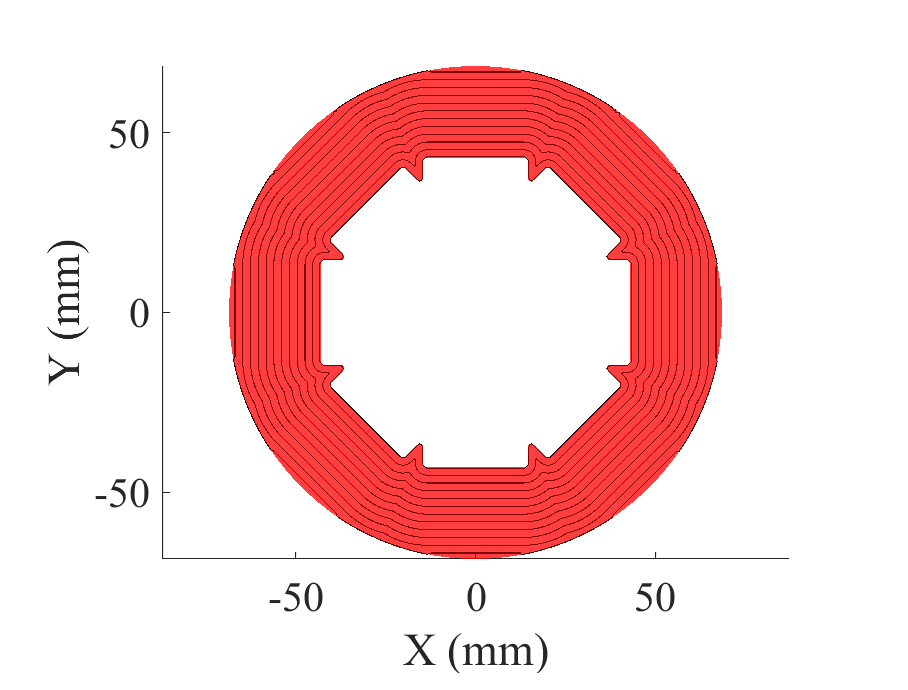
\includegraphics[width=0.7\linewidth]{LevelSet_Figures/FinocylBurnback.eps}
    \caption{Finocyl Grain. Burnback isocontours in 2mm steps}
    \label{fig:finocylgrainshape}
\end{figure}

The burning area vs the over all regression is displayed below for a cylindrical grain. The initial burn area is quite low and then increases to a much larger area. This can lead to having lower thrust in the start of the burn phase. A more extensive design could allow for a longer burn and also better flight control. This cylinder design has the same amount of cross sectional burn area in the beginning of the flight as the finocyl burnback plot shown later in this section. 

\begin{figure}[H]
    \centering
    \includegraphics[width=0.7\linewidth]{CombustorDesign/cylindricalgrainburnback.png}
    \caption{Cylindrical grain burnback}
    \label{fig:cylindricalGrainBurnback}
\end{figure}

The next figure is representative of the Finocyl burn area vs. regression. This is a much healthier trending line as the thrust is more constant. There should still be work done to attempt to get a more constant line and remove the dip that occurs in the middle but as can be seen this is a preferred grain shape. The initial burn area of the finocyl shape is much higher than that of the cylindrical one. This allows for higher thrust at the initial burn phase which in turn would allow the SFRJ to make quicker turns and pivots in order to have more control right after the separation of the booster.

\begin{figure}[H]
    \centering
    \includegraphics[width=0.7\linewidth]{CombustorDesign/finocylgrainburnback.png}
    \caption{Finocyl grain burnback}
    \label{fig:finocylGrainBurnback}
\end{figure}

The take away for the next step in the fuel grain shape will just be finalizing the grain. If a finocyl shaped grain continues to be the main choice, then the more intricate design choices will need to be made. In the burnback videos of the grains, it is apparent that the current finocyl shape burns a way at the corner of the pockets too quickly. This needs to be solved by either rounding the ports or by changing the port shape. The pointed cusps on the ends of the ports need to be changed. It is unlikely to actually get a pointed cusp in the fuel tank and thus simulating a point such as that can have misleading results. For the final finocyl grain runs, there was a slight arc cut into all of the pointed cusps to give the effect of having them all being curved and not directly pointed. 

\subsection{AeroValve}
\subsubsection{AeroValve Design - Coby Jacobs}
\label{AeroValveDesign}
The AeroValve is a unique feature to this SFRJ. This component came from the goal to decrease the velocity of the axial flow in the combustion chamber. The axial flow needs to be controlled in the combustion chamber to enhance flameholding capabilities. Specifically, if the Mach number in the chamber reached 0.76 the flame would extinguish. With the AeroValve, the flow from the inlet is separated, allowing for some axial flow in the combustion chamber and bringing some of the air through the AeroValve so that it can be distributed radially to slow down the flow and improve flameholding. The system is designed such that 40\% of the air is allowed to flow from the inlet into the combustion chamber and 60\% of the air flows into the AeroValve.The AeroValve has four injection port locations plus and end port. The injection ports are evenly distributed along the AeroValve. Fig. (\ref{fig:isometric}) shows an isometric view of the AeroValve, Fig. (\ref{fig:intake}) shows a view of the AeroValve intake, and Fig. (\ref{fig:bypassflow})

\begin{figure}[H]
    \centering
    \includegraphics[width=0.7\linewidth]{Combustor_Figures/isometric.png}
    \caption{AeroValve isometric view}
    \label{fig:isometric}
\end{figure}

\begin{figure}[H]
    \centering
    \includegraphics[width=0.7\linewidth]{AeroValve_Figures/bypass_intake.png}
    \caption{AeroValve intake}
    \label{fig:intake}
\end{figure}

\begin{figure}[H]
    \centering
    \includegraphics[width=0.7\linewidth]{AeroValve_Figures/bypass_flow.png}
    \caption{AeroValve flow}
    \label{fig:bypassflow}
\end{figure}

The AeroValve provides throttling by consisting of two concentric tubes, each with slots that can be aligned by the inner tube rotating a prescribed set of degrees to provide the needed mass flow. There are three scheduled settings for the position of the inner tune at ignition, cruise, and maneuver. 

The AeroValve was sized for the flow in the inner tube to be Mach 0.8. The inner diameter of the central valve for this condition is 1.43".  

\begin{figure}[H]
    \centering
    \includegraphics[width=0.7\linewidth]{Combustor_Figures/topview.png}
    \caption{AeroValve top view}
    \label{fig:topview}
\end{figure}

\subsubsection{AeroValve Actuation - Coby Jacobs}

In order to rotate the central tube of the AeroValve system, a gear actuation system had to be designed. The requirements of the actuation system were derived from eq. (\ref{torque_1}). It is assumed that there is negligible friction force between the two valves due to the use of bearings.

\begin{equation}
\centering   
\tau=I\alpha
\label{torque_1}
\end{equation}

This equation was be integrated twice with respect to time to so that a prescribed angle to rotate and time could be used to calculate torque.

\begin{equation}
\centering   
\tau=\frac{2I\alpha}{t^2}
\end{equation}

The moment of inertia of the valve was found using eq. (\ref{moment_inertia}).

\begin{equation}
    \centering
    I = \frac{\pi\rho h}{2}(r_2^4-r_1^4)
    \label{moment_inertia}
\end{equation}

Initially assuming that the tube would be made of steel and would have the maximum allowable dimensions in the chamber, the moment of inertia was estimated to be 0.01205 $kg-m^4$. Using this, a basic assumption to turn $60\deg$ in one second, and a large factor of safety, the required torque is 0.1 N-m, or .074 ft-lbs.

With a relatively small torque requirement, a small stepper motor can be used to control the gears. A large gear can be fitted around the AeroValve, but because the motor is much smaller than the large gear, the largest gear that can fit on the motor to be the driving gear will not be large enough to come in contact with the large driven gear. Due to this, future work will need to be done in the detailed mechanical design of the gear train so that a third gear can be fitted into the system.

\subsubsection{AeroValve Flow Analysis-Ariana Martinez}
The AeroValve flow analysis was divided between axial flow going through the AeroValve tube, and radial injected flow going into the combustor. both flows were analyzed under the assumptions of 1-D steady state incompressible flow with constant temperature. It is acknowledged that the initial mach in the AeroValve tube is 0.8 and incompressible flow is a poor assumption to make. However, the purpose of doing and analysis on the AeroValve was to assess its impact on the overall flight performance and thus it was desired to have a set of equations that could be solved analytically within the simulator. Due to having split mass flows, characterization of the AeroValve flow with compressibility effects will need to be conducted using a 2-D CFD model.This is an area of future work. A control volume of the axial flow is shown below in fig. \ref{fig:AeroValveAxialCV}.

\begin{figure}[H]
 \centering
    \includegraphics[width=0.5\linewidth]{AeroValve_Figures/AeroValveAxialCV.PNG}
    \caption{AeroValve Control Volume}
    \label{fig:AeroValveAxialCV}
\end{figure}

In this control volume, \textit{i} is a differential step down the combustor. The bypass analysis was discretized down the combustor and performed in tandum with the descrized combustor analysis.At the inlet of the AeroValve tube, \(i=1\),mass flow into the AeroValve,\(\dot{m}_{av}\) is set by
\begin{equation}
    \centering
    \dot{m}_{av}=Percent Bypass*\dot{m}_{inlet}
\end{equation}

The optimal percent of air bypassing the combustor to flow into the AeroValve was determined from paramater sweeps to be 60\% bypass. The pressure,\(P_{av}\), temperature, \(T_{av}\), velocity, \(v_{av}\),and density,\(\rho_{av}\) were set equal to corresponding inlet conditions.  

The injection mass flow rate, \(\dot{m}_{inj}\) going out of each injection port was set as the desired percentage of AeroValve flow to be distributed to each port. If there is no port at a location, \textit{i}, then injection mass flow percentage is set to zero. Eq.(\ref{mdot injection}) shows how each injection mass flow is calculated, where each element in the array represents the location corresponding to \textit{i} along the combustor.  
\begin{equation}
    \centering
\dot{m}_{inj}= \dot{m}_{av}*
[0 \hspace{2mm} 0 \hspace{2.5mm} \% \hspace{0.5mm} port \hspace{0.5mm} 1 \hspace{2.5mm}
 0 \hspace{2mm} 0 \hspace{2.5mm} \% \hspace{0.5mm} port \hspace{0.5mm} 2 \hspace{2.5mm}
 0 \hspace{2mm} 0 \hspace{2.5mm} \% \hspace{0.5mm} port \hspace{0.5mm} 3 \hspace{2.5mm}
 0 \hspace{2mm} 0 \hspace{2.5mm} \% \hspace{0.5mm} port \hspace{0.5mm} 4 \hspace{2.5mm} 
 0 \hspace{2mm} 0 \hspace{2.5mm} \% \hspace{0.5mm} end  \hspace{0.5mm} port]
 \label{mdot injection}
\end{equation}
The design criteria for determining a desired flow distribution through each port will be discussed the the Actuation Schedule section.
Thus, mass flow in the aerovalve tube at each location was calculated by mass conservation in eq.(\ref{bypass mdot})
\begin{equation}
    \centering
    \dot{m}_{av_{i+1}}= \dot{m}_{av_{i}}- \dot{m}_{inj_{i}}
     \label{bypass mdot}
\end{equation}
and velocity in the AeroValve at each port location, \(v_{av_{i+1}}\) is given by Continuity in eq.(\ref{bypass velocity}), where \(A_{av}\) is the cross sectional area of the inside of the bypass tube, and \(\rho_{air}\) is the air density at the end of the inlet.  
\begin{equation}
    \centering
    v_{av_{i+1}}= \frac{\dot{m}_{av_{i+1}}}{A_{av}\rho_{air}}
    \label{bypass velocity}
\end{equation}
it was assumed that there was no work or heat transferred in or out of the system. Thus, if \(\dot{m}_{inj}\) at a location \textit{i} was zero, then the static pressure in the Aerovalve tube, \(P_{av}\) at each location is given by eq.(\ref{bypass pressure 1})

\begin{equation}
    \centering
    P_{av_{i+1}}=P_{av_{i}}
\end{equation}
if \(\dot{m}_{inj}\) is nonzero at \textit{i}, then momentum balance on the control volume states:
\begin{equation}
    \centering
    P_{av_{i+1}}=P_{comb_{i}}
    \label{bypass pressure 1}
\end{equation}
where \(P_{comb}\) is the combustor static pressure at the location, \textit{i}.

Characterizing the flow properties down the Aerovalve tube allows us to characterize the flow of injected air into the combustor. The control volume for injected air is shown below in fig.\ref{fig:AeroValveInjectionCV}.

\begin{figure}[H]
 \centering
    \includegraphics[width=0.5\linewidth]{AeroValve_Figures/AeroValveInjectionCV.PNG}
    \caption{Injection Port Control Volume}
    \label{fig:AeroValveInjectionCV}
\end{figure}
it is assumed that in the AeroValve, radial velocity, \(v_{radial}\)is zero. because of the incompressible flow assumption, the radial velocity of injected mass flow from the AeroValve into the combustor,\(v_{inj}\) can be computed at a location,\textit{i} using eq.(\ref{discharge vel})

\begin{equation}
    \centering
    v_{inj_{i}}=\sqrt{2\rho_{air}(P_{av_i}-P_{comb_i})}
    \label{discharge vel}
\end{equation}
The injection port area,\(A_{inj}\), can then calculated at each location to accommodate the desired mass flow using Continuity in eq.(\ref{discharge area})
\begin{equation}
    A_{inj_i}=\frac{\dot{m}_{inj}}{\rho_{air}v_{inj_i}}
    \label{discharge area}
\end{equation}
These equations for solving the axial and radial flow of air in the AeroValve are looped in the simulator both down the combustor and with time. At each iteration down the combustor, the injected air mass flow is passed to the combustor code and the flow properties in the combustor are updated.

\subsubsection{Actuation Schedule-Ariana Martinez}
In order to meet all design requirements, it was desired to have airflow that was optimized for each state of flight. the flight states that were identified were ignition state, cruise state, and maneuver state\newline
\newline
    \underline{ Ignition State}\newline
    the goal during ignition was to be able to sustain the flame. this was achieved by injecting a large amount of radial flow in the front of the combustor in order to create re-circulation  of the flow. Flameholding will be discussed in detail in section V.C. Based on this criteria, the distribution of flow through the Aerovalve was selected to be 80\% of air through port 1, 20\% of air through port 2, and all other ports closed.fig.(\ref{fig:unrolled ignition}) shows the hole pattern for ignition phase
\begin{figure}[H]
\centering
  \includegraphics[width=.8\linewidth]{AeroValve_Figures/unrolled_aerovalve_ignition.PNG}
  \caption{Unrolled image of AeroValve Port Alignment during ignition}
  \label{fig:unrolled ignition}
\end{figure}
the corresponding mass flow rates and port sizes are shown below in fig.(xx) and fig. (xx) respectively. 
\begin{figure}[H]
\centering
\begin{minipage}{.5\textwidth}
  \centering
    \includegraphics[width=.8\linewidth]{AeroValve_Figures/ignition_port_areas.PNG}
  \captionof{figure}{AeroValve Mass Flow Schedule During Ignition}
  \label{fig:ignition mass flow}
\end{minipage}%
\begin{minipage}{.5\textwidth}
  \centering
  \includegraphics[width=.8\linewidth]{AeroValve_Figures/unrolled_aerovalve_ignition.PNG}
  \captionof{figure} Port Areas During Ignition Phase}
  \label{fig:ignition port area}
\end{minipage}
\end{figure}




the flow properties for the aerovalve and combustor in the ignition phase are shown below in figs. (xx) and (xx)



-ignitor goal and method
-image of rolled out aerovalve
-mass flow and velocity plots
-table of injection areas

-cruise goal and method
-image of rolled out aerovalve
-mass flow and velocity plots
-table of injection areas

-maneuver goal and method
-image of rolled out aerovalve
-mass flow and velocity plots
-table of injection areas

\subsubsection{AeroValue Thermal Analysis-Jonathan Rohwer}

Combustors are extreme environments and building an AeroValve to withstand the temperatures requires an understanding of the heat transfer into and out of the AeroValue. Using the thermal and transport properties from the AeroValue and combustor analysis a steady state solution was found. This solution has a couple of assumptions to simplify the initial analysis: \\
\begin{enumerate}
    \item Neglect axial heat conduction
    \item Neglect radiation
    \item Steady state
    \item Axisymmetric heat transfer
    \item Constant combustor port area \\
\end{enumerate}
The system was modeled as a solid pipe with convective flow on the inside (AeroValve flow) and outside (combustor). For the AeroValve flow, the McAdams pipe flow correlation was used to determine the convective heat transfer coefficient. This equation can be seen in eq.(\ref{McAdams})
\begin{equation}
    h_g=\frac{k_\infty}{D}0.026Re^{0.8}Pr^{0.4}
    \label{McAdams}
\end{equation}
where
\begin{equation}
    Re=\frac{\rho_\infty\nu_\infty D}{\mu_\infty}
\end{equation}
\begin{equation}
    Pr=\frac{\mu_\infty C_{p\infty}}{k_\infty}
\end{equation}
For the combustor flow, a form of the Bartz correlation was used to determine the convective heat transfer coefficient. This equation can be seen in eq.(\ref{Bartz})
\begin{equation}
    h_g=\frac{0.026}{D_h^{0.2}}\Big(\frac{\mu^{0.2}C_p}{Pr^{0.6}}\Big)_0(\rho_\infty U_\infty)^{0.8}\frac{1}{\sigma}
    \label{Bartz}
\end{equation}
where
\begin{equation}
    \sigma=\Big[\frac{1}{2}\frac{T_w}{T_0}\Big(1+\frac{\gamma-1}{2}M^2\Big)+\frac{1}{2}\Big]^{0.68}\Big[1+\frac{\gamma-1}{2}M^2\Big]^{0.12}
\end{equation}
\begin{equation}
    Pr=\frac{\mu_0 C_{p0}}{k_0}
\end{equation}
For Bartz specific units are used:
\begin{itemize}
    \item $C_p=[Btu/lb-\cr F]$
    \item $D_h=[in]$
    \item $T_w=T_0=[\cr R]$
    \item $\rho_\infty=[lb/in^3]$
    \item $U_\infty=[in/s]$
    \item $\mu=[lb/in-s]$
\end{itemize}


\subsubsection{Future Work - Stephen Kubicki}

An alternate design was created for the AeroValve as a potential lighter weight solution, but was not able to be integrated into the GLD simulation as of this paper's writing. A CAD rendition of this design can be seen in Fig. \ref{fig:AeroValve2_Labeled}. The design features rotating and stationary plates at the middle and end of the AeroValve, which control how much flow is apportioned in the fro

Approximate streamlines can also be seen in the figure, drawn in blue and going through the tube perforations.

\begin{figure}[H]
\centering
\includegraphics[width=1\textwidth] {AeroValve_Figures/AeroValve2_Labeled.png}
\caption{AeroValve Design Alternative}
\label{fig:AeroValve2_Labeled}
\end{figure}

\subsection{Flameholding-Ariana Martinez}

-equation and description
-image
-comments on equation
-velocity plots
-reflection


\input{CombustorDesign/Igniter.tex}

\subsection{Fuel Additives} 
\subsubsection{Background and Motivation}
The baseline fuel for design of the vehicle was neat HTPB, however Boron as a fuel additive was investigated for further performance improvement. Boron was chosen for further investigation due to its extremely high volumetric energy density and low toxicity compared to many conventional modern propellants. \\ \indent
Boron and its derivatives have been investigated for use in rockets since the 1950's, however neat boron has been plagued by ignition and combustion difficulties. John D. Clark, author of \textit{Ignition!: An informal history of rocket propellants}, was once asked for his definition of an exotic fuel to which he responded "It's expensive, it's got boron in it, and it probably doesn't work". However, recent advancements and new thinking, principally in the addition of the AeroValve, has improved our ability to burn Boron and advanced the state of Born combustion research. \\ \indent
The earliest recorded use of Boron in a ducted rocket flight vehicle was from the Augmented Thrust Propulsion (ATP) missile program from 1965-1971 [Keirsey]. Fuel loading's up to 60\% were investigated with claimed efficiencies as high as 90\%. The system was constructed from four individual inlets, combustors and exit nozzles. A single propellant grain was burned in a center blast tube and fed each combustor with hot boron-rich flows. 
\\ \indent
The United States Air force continued Boron solid fuel testing at the component level with the Boron Solid Fuel Ramjet (BSFRJ) and Boron Engine Component Integration, Test and Evaluation (BECITE) programs. Germany has also investigated Boron for flight vehicles, using a Boron-based fuel on the Anti Radiation Missile with Intelligent Guidance and Extended Range (ARMIGER). All of these vehicles, with the exception of BSFRJ, have been based on the Integral Rocket Ramjet model (IRR). An IRR combines the boost propellant chamber and ramjet fuel in a single continuous combustor which aids the combustion of Boron. The IRR chamber extends the mixing region, and in some vehicles provides extra burning oxidizer from the boost motor grain which significantly helps with combustion of the boron particles. \\ \indent
Literature indicates that the principle challenge in sustained ignition of boron particles occurs due to the two separate stages of combustion. First the particle ignites and the layer of $B_2O_3$ is removed, then the exposed born layer is burned. For optimal performance efficiency, the $B_2O_3$ must be recodensed before the nozzle. The performance limits lend themselves to needing three distinct conditions.
\begin{enumerate}
    \item High temperature initial to shed to outer layer of $B_2O_3$.
    \item High O/F to burn the exposed boron
    \item Low enough temperature to recondense the $B_2O_3$ back into a liquid state
\end{enumerate}
Conditions 1 conflict with conditions 2 and 3, as O/F increases from optimal temperature will decrease. \\ \indent
There exists some debate within the SFRJ community as to which global reaction rate model to use and two primary models have been developed and discussed. The first model, proposed by King in 1972, and the second model, originally proposed by Glassman and updated by Li and Williams in 1990, primarily differ in how they consider the heterogeneous reactions occurring on the particle surface. We chose to work with the King model, to align results with earlier analytical and experimental work by Benni Natan at Technion.
\subsubsection{Combustion Model}
In order to evaluate Boron as a potential SFRJ additive, a method of determining the combustion efficiency is required. We developed a code which calculates the reaction rate of a Boron particle in a SFRJ flow field. The 1D model considering the effect of flow temperature and composition to determine the diameter of a Boron particle at a specific axial location and moment in time. \\ \indent
Natan notes that there is a strong dependence on the ejection velocity of the fuel surface due to the particle crossing the flame boundary zone, and thus built his model in 2D to account for this. Due to computational limits, we limited our analysis to 1D. We assumed that the initial temperature of the Boron particle was 800$^{\circ}$ which account for preheating of the fuel before the Boron particle is entrained in the flow field. We also assumed that a released particle would start at 5 m/s and aerodynamic effects would increase particle speed until it matched the gas flow speed. However, the model is very insensitive to this initial speed because the released particle reaches flow velocity very quickly. Lastly, the flow temperature of Boron was calculated in CEA assuming complete combustion. Although CEA is not an especially useful tool with Boron because it cannot account for unburned products, it did allow us to calculate an approximate gas temperature. \\ \indent
The governing equations were based on the work of King and primarily considered the thermolysis and hydrolysis of the $B_2O_3$ shell, and combustion of the exposed Boron with $O_2$ in the chamber. 
\subsubsection{Bypass Usage}
Due to the aforementioned complications with Boron combustion, innovative solutions are required. One such solution involves a bypass flow redirected and dumped directly in an aft mixing chamber. This bypass flow has two purposes, firstly it ensures that any unburned Boron particles have ample $O_2$ to complete combustion. And secondly, it cools the particles enough to recondense $B_2O_3$ and ensure that maximum energy is extracted from the fuel formulation. However, this method requires a larger inlet in order to justify the high percentage of flow not being combusted. \\ \indent
In order to improve the bypass air concept, the team created the AeroValve which redirects bypass air into the chamber at discrete points. This allows further control of the $O_2$ content withing the chamber. With proper optimization of valve control, a high percentage of the boron could be burned and $B_2O_3$ recondensed in order to improve performance. \\ \indent
\subsubsection{Manufacturing}
\subsubsection{Results}
Two sets of results were produced which demonstrate the efficiency of combustion in the chamber and a second set which demonstrate the theoretical performance of Boron in the flight vehicle. Future work to integrate the models and determine the actual performance is required. \\ \indent
As seen below in figure
\subsubsection{Future Work}
Experimental work is required to further the development of additives in SFRJ's. Though considerable issues occur with boron combustion, experiments with new bypass techniques such as the AeroValve, may be able solve these problems. \\ \indent
Further investigation into other additives to improve performance. The SFRJ did not suffer from a low thrust force as is often seen in hybrid rockets, so additives which improve regression will not help performance as much as those that improve Isp. \\ \indent
An additional option is investigate oxidizer additives to improve the oxidizer content in the chamber. If added in low enough quantities to not be self-sustaining, they present a safe and economic method to improve performance.




% Nozzle Design
\section{Nozzle Design}

\subsection{Trade Study}

\subsection{Design Overview}

\subsection{Analysis \& Sizing}

\subsection{Future Work}

% Airframe Design
\section{Airframe Design}

\subsection{Buckling Analysis - Silas Meriam}


\subsection{Internal Pressure Analysis - Silas Meriam}


\subsection{Sensor Package and Control Unit - Silas Meriam and Melanie Grande}
For mass and volume sizing purposes, Guidance, Navigation, and Control (GNC) and Power units were investigated for the GLD. The GLD can be controlled by a small logic board, for example an ODROID-XU4, which has DC Voltage 5 V and weighs merely 1.5 oz. Power can be supplied by a Lithium Polymer (LiPO) battery pack, for example the Tenergy 900 mAh 7.4 V 25C LiPO Battery, which weighs approximately 1.6 oz. Transformers and wiring would be included as necessary and are estimated to weigh approximately 3 oz. This GNC and Power design should allow approximately three minutes minimum operational time with fully loaded actuators, which is plenty for our GLD, whose SFRJ stage burns for nearly 30 s. 

\color{red}TODO: Add discussion/CAD about the sensor package in the nose.\color{black}

% Fin Design
\section{Fin Design}

\subsection{Trade Study}

Multiple attitude control methods were considered for the GLD design including jet tabs, jet vanes, and external fins. An overview of each of these concepts is shown in Figures \ref{fig:atitudectrl_conc}.

\begin{figure}[H]
    \centering
    \begin{subfigure}[b]{0.3\textwidth}
        \centering
        \includegraphics[height=1.2in]{AtitudeControl_Figures/fins.png}
        \caption{Fins}
    \end{subfigure}
    ~
    \begin{subfigure}[b]{0.3\textwidth}
        \centering
        \includegraphics[height=1.2in]{AtitudeControl_Figures/tabs.png}
        \caption{Jet Tabs}
    \end{subfigure}
    ~
    \begin{subfigure}[b]{0.3\textwidth}
        \centering
        \includegraphics[height=1.2in]{AtitudeControl_Figures/vanes.png}
        \caption{Jet Vanes}
    \end{subfigure}
    \caption{Overview of attitude control system concepts \label{fig:atitudectrl_conc}}
\end{figure}

Missiles that utilize fins for attitude control are typically comprised a set of static fins and a set of maneuverable fins. The static fins are designed to help control the location of the vehicles center of pressure over its operational envelope while the maneuverable fins provide the control torque about the center of gravity. The fin control scheme can be configured such that the maneuverable fins are located forward of the vehicle center of gravity or such that the maneuverable fins are located aft-ward of the center of gravity. Tail control provides better control authority at high angles of attack in comparison to canard control and typically is used in long range applications. Conversely, canard (forward) control is better for low angle of attack and short range applications. Since the SFRJ design will be performing aggressive maneuvers and is designed to maximize range, only tail control was considered when trading fins against other concepts.

The jet tab concept operates by obstructing the nozzle exhaust flow with blunt bodies which alters the effective thrust vector angle of the vehicle. This concept is attractive due to its simple and low power construction and because it does not generate any performance loss for the vehicle when it is not being used. However, thrust losses of are predicted to be a maximum of approximately 5\% for our application \cite{eatough1977} with limited control authority especially in the roll axis when compared to the fin design.

Jet vanes present a hybrid approach between the jet tab and fin designs. Maneuverable fins are located in the nozzle exhaust stream to control the thrust vector. This approach provides limited advantages over the jet tab and fin methods due to the large performance losses that it induces, its high power requirements, and complexity to design. Due to these disqualifying limitations, the jet vane concept was not considered during final attitude control method selection.

Power, complexity of design, control authority, performance loss, and mass were the prime factors considered in the final design selection. To accurately compare the jet tab and tail fin approaches, a preliminary design was generated for each method. CAD renders of the two designs are displayed in Figure \ref{fig:atitudectrl_prel} below. The fin design consists of four fins with a angle of attack range from -5$^\circ$ to 5$^\circ$. Each fin is driven by a single electrical actuator with a 1.575 inch moment arm. The jet tab design is comprised of four sets of two jet tabs. The tabs in a set rotate counter to each other and are driving by two DC motors on a single gear train. The performance of the fins was characterized with linear supersonic theory while the jet tab design was characterized using empirical data from previous designs \cite{eatough1977}. When these two preliminary designs were compared, it was determined that while the fin design requires twice as much electrical power as the jet tabs, it also provides better control authority, was lower mass, and required a simpler mechanism design. It is for these reasons that the tail fin control scheme was selected for the GLD design.

\begin{figure}[H]
    \centering
    \begin{subfigure}[b]{0.45\textwidth}
        \centering
        \includegraphics[width=3.0in]{AtitudeControl_Figures/fin_design.png}
        \caption{Tail Fins}
    \end{subfigure}
    ~
    \begin{subfigure}[b]{0.45\textwidth}
        \centering
        \includegraphics[width=2.75in]{AtitudeControl_Figures/tab_design.png}
        \caption{Jet Tabs}
    \end{subfigure}
    \caption{Preliminary Attitude Control Concepts \label{fig:atitudectrl_prel}}
\end{figure}

\pagebreak

\subsection{Design Overview}

\begin{multicols}{2}

    \begin{wrapfigure}{R}{0.5\textwidth}
        \begin{center}
        \includegraphics[width=\linewidth]{AtitudeControl_Figures/fin_int_design.png}
        \end{center}
        \caption{Integrated Fin Design \label{fig:fin_int_design}}
    \end{wrapfigure}
\end{mui

\subsection{Analysis \& Sizing}

\subsection{Future Work}

% Modeling and Simulation
\section{Modeling and Simulation}

% Performance
%\subsection{Performance}
%\subsection{Combustor Modeling and Simulation - Jordan Fisher} \label{CombustorModelingAndSim}
The combustor is a key component to be simulated to estimate performance of the SFRJ. As the vehicle flies, the combustor experiences transients in many operating parameters which must be taken into account accurately. To allow for simulation a discretized combustor model has been developed which takes into account mass addition, combustion, area change, and flow properties down the length of the fuel grain. The combustor flowpath simulation is built as an independent function in the simulator environment so it can be used with any arbitrary fuel grain arrangement, and analyzed while coupled with an inlet and nozzle or simulated on its own. A flowchart of the combustor flow path loop is shown in Fig. \ref{fig:flowpath}. \\ \indent

\begin{figure}[hbt]
\centering
\includegraphics[width=1\textwidth] {Combustor_Figures/flowpath.PNG}
\caption{Combustor Flowpath Loop}
\label{fig:flowpath}
\end{figure}

To begin the flowpath simulation, flow properties are taken as inputs. To fully define the flow, the properties that need to be defined are mass flow rate, temperature, pressure, gamma, Cp, and molecular weight. For the SFRJ simulation, mass flow rate, stagnation temperature and pressure are taken from the output of the inlet object. Molecular properties are taken from air since no chemical reactions are occuring until the combustor is simulated. To iterate along the length of the fuel grain, the combustor port is estimated as a series of discrete control volumes as seen below in Fig. \ref{fig:controlvolume}\\ \indent

\begin{figure}[hbt]
\centering
\includegraphics[width=.5\textwidth] {Combustor_Figures/grain_sections.PNG}
\caption{Differential Combustor Port Element}
\label{fig:controlvolume}
\end{figure}

At the beginning of each differential port section, fuel mass flow rate is calculated according to the equation $\dot{m}_f=r_b  \rho  A_b$, where $\dot{m}_f$ is the mass flow of fuel into the port, $r_b$ is the fuel grain burnback rate in meters per second, $\rho$ is the fuel grain density and $A_b$ is the burn area of the fuel grain exposed to the flow. These three fuel grain properties are known inputs in the flowpath loop calculated from the previous time step. Their calculation is discussed in the subsequent sections. At each section of the port there is also the possibility of mass injection of air through the use of the AeroValve component. Flow entering the combustion chamber is diverted to a smaller tube and allowed to pass back into the port through a series of orifices. The mass flow of air entering the combustor is computed using the pressure in the aerovalve along with incompressible orifice flow calculations. With the continuity equations for mass balance satisfied for the discrete grain section, the simulation of combustion can begin. OF is calculated as a cumulative Oxidizer - to - fuel ratio based on the total mass flow in the port to all of fuel that has entered the port. This OF is put into a CEA calculation for estimation of the reactions occuring between the incoming air and the fuel grain. With the implementation of a native CEA runner in MATLAB the computational cost of running  a full chemical simulation is mitigated. The stagnation temperature due to combustion, as well as the new $\gamma$, Cp, and molecular weight due to reactions is taken from the output of the CEA simulation. Using equations derived in \cite{hyball}, conservation of momentum and energy can be applied to the differential port section to iterate to the new mach number and pressure in the port. The equations used for this analysis are shown below.  \\ \indent

\begin{equation}
\centering   
\frac{dM}{M}=F_1 (\frac{dH}{C_pT}+\eta\frac{d\dot{m}}{\dot{m}}-\frac{dMw}{Mw})-.5\frac{d\gamma}{\gamma}
\end{equation}

\begin{equation}
\centering   
\frac{dP}{P}=F_2 (\frac{dMw}{Mw}-\frac{dH}{H}-2\eta\frac{d\dot{m}}{\dot{m}}) 
\end{equation}
where
\begin{equation}
\centering   
\frac{dH}{C_pT}=\frac{d(C_pT_c)-(dC_p)\Bar{T}}{C_pT}
\end{equation}

\begin{equation}
\centering   
F_1=.5\frac{1+\gamma M^2}{1-M^2}
\end{equation}

\begin{equation}
\centering   
F_2=\frac{\gamma M^2}{1-M^2}
\end{equation}

\begin{equation}
\centering   
\eta=1+\frac{\gamma-1}{2}M^2
\end{equation}

With all of these steps we are able to track the pressure, temperature, mach number, and mass flow along the length of the combustion chamber. After the flowpath is simulated the mass flow and port area are known at each discrete location and known. With these variables, the fuel burn rate can be computed for the next time step using the equation $r_b=aG_{Ox}^n$, where a is the burn rate coefficient, .49 mm/s and n is the burn rate exponent, .61. $G_{Ox}$ is the port mass flow per unit area. The regression model and coefficient models are determined experimentally for HTPB in \cite{Pourpoint}. The SFRJ performance sensitivity to inaccuracies in the burn rate coefficients is discussed in a later section. \\ \indent

To simulate the full flight vehicle properly, there must be mass flow continuity through the full flow path of the system from inlet, through the combustor and aerovalve, and through the nozzle. The flow in each of these sections must have cross-talk so that mass flow is conserved properly and flow does not choke or unchoke at the wrong location. The mass flow rate and total temperature entering the vehicle is set by the flight mach number and the inlet capabilities. These are treated as fixed inputs. The pressure at the start of the combustor is an unknown parameter. To ensure proper choking at the nozzle throat after the combustor, an iterative solving loop is implemented. This solving loop pre-populates the combustor flowpath function and solves for the flow along the length of the fuel grain. It then checks if the flow is properly choked at the nozzle throat. If the flow is not choked properly, the pressure guess is changed successively until the throat is choked. This final pressure value is saved and used as the initial pressure guess for the next time step of the simulation. In a physical sense, this pressure solving loop represents the shock train in the inlet needing to respond to the downstream conditions in the combustor to satisfy continuity. If the pressure needed to choke the nozzle throat becomes too high for the inlet to provide, the inlet unstarts and the simulation fails for current design conditions. At the end of the combustion simulation at each time step the fuel burn rate is used to update the fuel grain geometry. With the simple cylindrical grain which was used for much of the simulations performed, an analytic equation for the burn area and port area as a function of grain burnback distance can easily be obtained. For more complex grain shapes such as a finocyl type, a code to generate a table of burn and port areas as a function of burnback is obtained from a custom-developed level-set code which is to be discussed in a later section. A flowchart of the full combustor simulation can be seen below in Fig. \ref{fig:timeloop}  \\ \indent


\begin{figure}[H]
\centering
\includegraphics[width=1\textwidth] {Combustor_Figures/timeloop.PNG}
\caption{Iteration of Combustor Properties over Time}
\label{fig:timeloop}
\end{figure}


The flight simulation of the SFRJ is a highly dynamic process, with environment variables such as flight speed, grain geometry, mass flow rate and aerovalve throttling changing constantly throughout the time that the combustor is burning. This can be observed in the plots of operating parameters down the length of the fuel grain at different snapshows during the burn. The first parameter tracked is the oxidizer to fuel ratio seen in Fig. \ref{fig:OF}. In this plot the different flight states can be seen. During the beginning of the burn, the aerovalve allows for air the be injected in the beginning of the fuel grain. This keeps the OF ratio high and allows for flame stabilization on the incoming jet of air. During the middle burn phase two small spikes in the OF ratio can be seen near 5 and 10 inches. This air injection facilitates a higher thrust level so that the vehicle can maintain its flight speed during maneuvers. At the end of the burn the grain begins to burn out from the rear sections.\\ \indent

\begin{figure}[H]
\centering
\includegraphics[width=1\textwidth] {Combustor_Figures/OF.png}
\caption{Oxidizer to Fuel Ratio in the Combustor}
\label{fig:OF}
\end{figure}

The same flight states previously described can also be seen well in the port mass flow plots shown in Fig. \ref{fig:massflow}. The large jumps in mass flow in the port can be attributed to discrete air injection locations allowed by the aerovalve to control thrust levels and fuel regression. The mach number plot in Fig. \ref{fig:mach} shows that at the beginning of the burn the mach number in the combustor reaches a maximum slightly above .5. This high speed flow emphasizes the need to take extra care in designing the flameholding sequence near ignition. As the fuel grain regresses the combustor port opens up and the mach number along the fuel grain length decreases significantly. The stagnation temperature and static pressure plots are shown in figures \ref{fig:temperature} and \ref{fig:pressure}, respectively. The maximum value in the temperature plots shows where the combustor is burning the most efficiently. After this point, extending the grain length any longer gives a decrease in efficiency for the system. For this reason it is desired to keep the grain length short enough that there is still enough oxygen left in the port near the aft end of the combustor so that nearly stoichiometric flame temperatures can be maintained.\\ \indent

\begin{figure}[H]
\centering
\includegraphics[width=1\textwidth] {Combustor_Figures/Massflow.png}
\caption{Mass Flow Rate in the Combustor}
\label{fig:massflow}
\end{figure}



\begin{figure}[H]
\centering
\includegraphics[width=1\textwidth] {Combustor_Figures/Mach.png}
\caption{Mach Number in the Combustor}
\label{fig:mach}
\end{figure}

\begin{figure}[H]
\centering
\includegraphics[width=1\textwidth] {Combustor_Figures/Temperature.png}
\caption{Stagnation Temperature in the Combustor}
\label{fig:temperature}
\end{figure}

\begin{figure}[H]
\centering
\includegraphics[width=1\textwidth] {Combustor_Figures/Pressure.png}
\caption{Static Pressure in the Combustor}
\label{fig:pressure}
\end{figure}

\subsubsection{Burn Rate Sensitivity Analysis - Jordan Fisher}
As stated previously, the fuel regression rate model was taken from \cite{Pourpoint}. This work presents empirical values for burn rate coefficients for HTPB burning in an oxygen environment in a hybrid rocket system. This application is similar to our SFRJ but cannot be fully trusted. Until experimental verification of the combustor code and burn rate coefficients can be performed, a key risk area of the design is inaccuracy of the burn rate model. A sensitivity analysis of the performance of the system was conducted to gauge the dependency of key flight parameters such as ground range, burn time, average thrust and vehicle flight mach number to the fuel grain burn rate coefficient and exponent. Results can be seen in Fig. \ref{fig:sensitivity}. The burn coefficients a and n were varied $\pm 10\%$ from the values prescribed in \cite{Pourpoint}. For most of the tested range of inputs, a variation of about 25\% can be seen in the ground range and burn time. Average thrust and flight mach number vary by a range of about 10\%. Below the solid black line seen on each plot is a region of unstarted operation. This area poses a greater risk to the performance of the system. Experimental verification of the combustor model will need to be conducted to anchor the flight performance predictions more accurately.  \\ \indent



\begin{figure}[H]
\centering
\includegraphics[width=1\textwidth] {Combustor_Figures/sensitivity.PNG}
\caption{Sensitivity Analysis of Various Performance Metrics}
\label{fig:sensitivity}
\end{figure}





%\subsection{Combustor Model Validation - Stephen Kubicki}
A lumped parameter combustor model was created as a validation tool for the discretized combustor model discussed in \ref{CombustorModelingAndSim}. An important step in the design was to ensure the discretized model is calculating combustor behavior appropriately and providing accurate data for the SFRJ flight simulation. The lumped parameter model serves as a reliable comparison as it is a simpler model based on a few presiding assumptions, listed below. 

\begin{enumerate}
  \item Mach number is low throughout the combustor
  \item Combustor can be characterized by a single pressure
  \item Fuel grain burns at a single regression rate \\
\end{enumerate}

These assumptions combined lead to an important simplifying model assumption: axial variations in flow properties down the length of the combustor are ignored, so the entire combustor can be characterized by a single set of flow properties that varies with time. This makes the lumped parameter model akin to a discretized combustor model with a single axial section, the length of the combustor. The lumped parameter model is in many ways similar to the discretized combustor model described previously; the simulation is built as an independent function in the simulator environment, follows a similar flowpath loop as shown in Fig. \ref{fig:flowpath} (however without bypass modeling), and follows the same exact time iteration/pressure solving loop as described in Fig. \ref{fig:timeloop}. The time iteration of the lumped parameter combustor model will not be discussed in detail due to its similarity to the discretized combustor model, but the process and equations utilized to compute the updated flow properties will be described below. 

The lumped parameter model first pulls in the flow properties exiting the inlet pipe (mass flow rate, temperature, pressure, molecular weight, ratio of specific heats, etc.) and sets those as the flow properties in the entire combustor. The port area is computed based on the grain geometry at the current time step, and the Mach number in the combustor is computed to check if the flow is choked. The fuel regression rate is then found based on the oxidizer mass flux through the combustor and the regression rate constants for HTPB, as dicussed in \textbf{Reference ???}. Fuel mass flow rate can then be calculated based on the regression rate, the fuel density, and the exposed grain burn surface area (based on the grain geometry at the current time step). The oxidizer to fuel ratio, or O/F, is computed so CEA can be called using O/F and the current flow properties to simulate combustion, outputting updated properties for the entire chamber. Finally, the new total mass flow rate is calculated to recheck if the combustor is choked. Since axial variations in flow properties are ignored, this outlined process is repeated for each time step, pulling the initial flow properties from the inlet pipe each time and updating the grain geometry between iterations. The equations that this process describes are listed below. 

\begin{equation}
\centering   
M=\frac{\dot{m}_{ox}\sqrt{\frac{RT}{\gamma}}}{pA_p}
\end{equation}

\begin{equation}
\centering   
r=aG_{ox}^n=a(\frac{\dot{m}_{ox}}{A_p})^n
\end{equation}

\begin{equation}
\centering   
\dot{m}_f=r\rho_fA_b
\end{equation}

\begin{equation}
\centering   
O/F=\frac{\dot{m}_{ox}}{\dot{m}_f}
\end{equation}

\begin{equation}
\centering   
[flow,T_o,\gamma,C_p]=CEA(T,p,\frac{p_c}{p_e},O/F)
\end{equation}

\begin{equation}
\centering   
\dot{m}_{tot}=\frac{\dot{m}_{ox}}{\dot{m}_f}
\end{equation}

\begin{equation}
\centering   
M=\frac{\dot{m}_{tot}\sqrt{\frac{RT}{\gamma}}}{pA_p}
\end{equation}

The two combustor models were run in a static test stand simulation rather than a flight simulation in order to isolate the behavior of the models as much as possible, giving the best comparison of true behavior. Running the models in a flight simulation would lead to exaggerated divergence in behavior due to extra degrees of freedom in flight conditions. For example, consider a case where the two models were run in flight simulations beginning at the same initial flight conditions. A difference in combustor behavior can lead to cascading differences through the following: combustor behavior, performance parameters (i.e. thrust), vehicle dynamics, flight conditions, and flow properties through the inlet assembly. This process repeats each time step, with the properties of the two models diverging increasingly further as time progresses. The benefit of running the two models on a test stand is that it provides constant inlet conditions, hence isolating any possibility of the aforementioned cascading differences. Additionally, the two models were run without an AeroValve due to the fact that the lumped parameter model does not take into account axial variations in flow, so injecting bypass flow is not possible. Therefore, AeroValve flow was omitted to keep comparisons of the governing equations as close to 1:1 as possible. Finally, since the lumped parameter model uses a single set of flow properties to characterize the entire combustor, a set of flow properties from a discretized combustor section were selected (the aft-most section) to compare against. Flow properties from the static test stand runs for each of the combustor models are shown in Fig. \ref{fig:LPA_1} - Fig. \ref{fig:LPA_3} below.

\begin{figure}[H]
\centering
\includegraphics[width=1\textwidth] {Combustor_Figures/LPA_1.png}
\caption{Lumped Parameter Model - Static Temperature (Left) and Static Pressure (Right) vs. Time}
\label{fig:LPA_1}
\end{figure}

\begin{figure}[H]
\centering
\includegraphics[width=1\textwidth] {Combustor_Figures/LPA_2.png}
\caption{Lumped Parameter Model - Mach Number (Left) and Mass Flow Rate (Right) vs. Time}
\label{fig:LPA_2}
\end{figure}

\begin{figure}[H]
\centering
\includegraphics[width=1\textwidth] {Combustor_Figures/LPA_3.png}
\caption{Lumped Parameter Model - O/F (Left) and Port Area (Right) vs. Time}
\label{fig:LPA_3}
\end{figure}

A quick glance at these plots may make it appear that there is a marginal difference between the property time histories for the lumped parameter cobustor model and the discretized combustor model, however a closer inspection of the y-axes makes it clear that the two models behave in fairly close agreement. The average difference between the two models' properties are displayed in Table \ref{tab:LPAvsDiscrete}.

\begin{table}
    \centering
    \caption{Combustor Property Differences Between Models}
    \begin{tabular}{c|c}
    \textbf{Property} & \textbf{Difference [\%]} \\
    \hline
        Static Temperature & 0.8 \\ 
        Static Pressure & 1.5 \\ 
        Mach Number & 4.0 \\ 
        Mass Flow Rate & 0.5 \\ 
        O/F & 2.5 \\ 
        Port Area & 0.1
    \end{tabular}
    \label{tab:LPAvsDiscrete}
\end{table}

The initial conditions of the properties differ due to innate differences between the two models, particularly due to the fact that the properties update down the combustor length in the discretized model. Importantly, the trends of the properties appear to be consistent across the models, with difference between some properties being consistent with time while the rest converge with time. This provides good confidence that the discretized combustor model is used correctly and captures the combustor behavior appropriately, ultimately validating the model. Additionally, the plot of port area vs. time (Fig. \ref{fig:LPA_3} on the right) shows that both models reach the maximum port area, i.e. burn out, at nearly the same time, further supporting the validation of the model. 

% Lift and Drag Analysis
\subsection{Lift and Drag Analysis}

\subsubsection{Lift Analysis - Thomas Satterly}

Lift is a complicated metric to calculate when in the early stages of design. For this analysis, a lift coefficient was approximated by using a cylindrical lifting body model \cite{fleeman_2001}, outlined in Equations \ref{eqn:normalCoeff} - \ref{eqn:lift}. In addition to the lifting body force, the lift coefficients of the movable and stationary fins, calculated using a CFD model, were added to create a final lift coefficient value. 

\begin{align}
    C_n &= \sin(2\alpha)\cos(\alpha/2) + 2 \frac{L_{cyl}}{D_{cyl}}sin(\alpha)^2
    \label{eqn:normalCoeff}\\
    C_L &= \cos(\alpha)C_n + C_{L, fins}
    \label{eqn:liftCoeff}\\
    L &= 0.5\rho V^2 S C_L
    \label{eqn:lift}
\end{align}


\subsubsection{Drag Analysis - Manav Vaghashiya}
Drag analysis is an important aspect of verifying the feasibility of the SFRJ design. Validation of the drag coefficient can be done by comparing the analysis at a specified Mach number against an existing design. This can provide insight into whether the design will satisfy its requirements and specifications. It is important to have an accurate and realistic drag coefficient since it affects the range of the SRFJ as well as other performance parameters. The complex design of the SFRJ posed an intricate challenge when conducting the analysis.

Drag analysis of the vehicle is divided into several components. Drag coefficients from Skin Friction Drag, Wave Drag, Body-Base Drag, Fin Drag, Inlet Cowl Drag and Inlet Spillage Drag are amalgamated to form the complete drag analysis of the vehicle. Each component or components is calculated using various sources of literature. Skin Friction Drag, Wave Drag and Body-Base Drag is calculated using literature from \textit{Tactical Missile Design} \cite{fleeman_2001}. Inlet Cowl Drag is calculated using “A Tool for the Aerodynamic Design and Analysis of Supersonic Inlets” and Inlet Spillage Drag is computed using “Supersonic Inlet Design.”

Skin Friction Drag is the drag created by the friction of air against the surface of the SFRJ. Wave Drag is the drag imposed on the SFRJ by the formation of shocks. Body- Base drag is the drag created tail end of the missile. Skin Friction Drag, Wave Drag and Body-Base drag is computed using several loops which consider the geometry of the vehicle as well as flow properties such as velocity. Inlet Cowl Drag is the drag caused by the shock created at the cowl and Inlet Spillage Drag is created by the “spillage” of air at the inlet of the SFRJ. Both, Inlet Cowl Drag and Inlet Spillage Drag is computed using 2-dimensional equations from literature that consider the geometry of the inlet and the flow properties at the inlet. Fin Drag is the drag produced by the fin and is calculated using CFD analysis of the fin and interpolating the data. 


\subsubsection{Results and Future Work}

The results of the lift calculation is presented in Figure \ref{fig:liftCoeff}. As expected, the lift coefficient is constant across a changing Mach number. While this is not representative of a real system, the effect of lift on the SFRJ is minimal due to flying at a low angle of attack, typically less than seven degrees.

\begin{figure}[H]
    \centering
    \includegraphics[width=0.7\textwidth]{LiftAndDragAnalysis/figures/LiftCoeffcAoA.png}
    \caption{Lift Coefficient vs. Angle of Attack}
    \label{fig:liftCoeff}
\end{figure}

The results of the drag analysis is shown in the Figure below. At mach 2.5, the SFRJ experiences a drag coefficient of 0.74. In comparison to Twin Intake X-Tail design, which has a drag coefficient of 0.56 at mach 2.5, the SFRJ designed experiences much higher drag values. Drag coefficient also increases as mach increase in the figure which is an unusual trend and thus needs further attention. 

\begin{figure}[H]
    \centering
    \includegraphics[width=0.7\linewidth]{LiftAndDragAnalysis/DragChart.png}
    \caption{Drag Coefficient vs Mach}
    \label{fig:Drag Coefficient}
\end{figure}

After further analysis of the results, higher drag coefficient and increasing drag  can be attributed to the 2-dimensional equations used to conduct the drag analysis of the Inlet. Since the Inlet has complex 3-dimensional geometry, further analysis using CFD will give a more accurate drag coefficient and thus reduce the overall drag coefficient. In future, further attention to Inlet Spillage Drag and Inlet Cowl Drag using CFD needs to be conducted. 

The drag polar is shown in Figure \ref{fig:dragPolar}. The results are generally as expected, with a peak lift-to-drag ratio near and angle of attack of 25 degrees. Increasing Mach number shows a decrease in the lift-to-drag ratio, which is contradictory to conventional knowledge, but this is a result of the deficiencies of the lift and drag models used. Overall, the peak lift-to-drag ratio approach 1.2, which is near a common approximation of 1.5 \cite{fleeman_2001}. 

\begin{figure}[H]
    \centering
    \includegraphics[width=0.7\textwidth]{LiftAndDragAnalysis/figures/DragPolar.png}
    \caption{Drag Polar}
    \label{fig:dragPolar}
\end{figure}



% Trajectory
\subsection{Trajectory - Thomas Satterly}

\subsubsection{Physics Integration Model}
The trajectory of the boosted stack and SFRJ is a natural fallout of the physics model interacting with attitude controllers and the calculated lift, drag, thrust, and gravity forces. A three-degrees-of-freedom point mass model was used in conjunction with a Runge-Kutta 4th order integrator, described in Equations \ref{eqn:RK4_1} - \ref{eqn:RK4_6} for simulating linear motion. The orientation vector, which is decoupled from the velocity vector out of a necessity to simulate pitch, roll, and yaw maneuvers, was handled outside of the physics integration by assuming constant turn rates for simplicity. 

\begin{align}
    y_{n+1} &= y_n + \frac{1}{6}(k_1 + 2k_2 + 2k_3 + k_4) 
    \label{eqn:RK4_1} \\
    t_{n+1} &= t_n + h 
    \label{eqn:RK4_2}\\
    k_1 &= hf(t_n, y_n) 
    \label{eqn:RK4_3}\\
    k_2 &= hf(t_n + \frac{h}{2}, y_n + \frac{k_1}{2}) 
    \label{eqn:RK4_4}\\
    k_3 &= hf(t_n + \frac{h}{2}, y_n + \frac{k_2}{2}) 
    \label{eqn:RK4_5}\\
    k_4 &= hf(t_n + h, y_n + k_3)
    \label{eqn:RK4_6}
\end{align}
\begin{align*}
y_n&: \text{Vehicle state}\\
t_n&: \text{Time}\\
h&: \text{Change in time}\\
f(t_n, y_n)&: \text{Change of state as a function of time and state}
\end{align*}

A time step convergence study was conducted by simulating a Cesaroni Pro150-40k 40960O8000-P boosting a small secondary stage that, once dropped at boost stage burnout, burns for and additional 5 seconds. The altitude and speed of the second stage was recorded and compared after 30 seconds of total simulation time. The results are shown in Figure \ref{fig:timeStepConvergence}.

\begin{figure}[H]
\centering
\includegraphics[width=0.75\textwidth]{ModelingAndSim/figures/timeStepConvergence.png}
\caption{Time Step Convergence. Solid lines denote a smoothed mean. Areas show 1$\sigma$ bounds}
\label{fig:timeStepConvergence}
\end{figure}

Results show that variation in Mach and altitude with a different time step sizes is drastically reduces at a time step of less than 0.1 seconds. It is also shown that the variation in Mach and altitude is less than 2 percent for a time step size of 0.25 seconds. For the the purpose this study, a 0.25 second time step will be used to balance computational speed and result quality.

\subsubsection{Control \& Maneuvers}

\paragraph{Launch \& Boost} The orientation of the vehicle during the launch and boost stages was held at a constant elevation angle of 35 degrees. This angle was chosen because it provided a balance between attaining a supersonic drop condition near Mach 2 while setting up the SFRJ stage at and altitude and attitude that made sustained combustion durning subsequent maneuvers feasible. A greater initial angle of attack would tend to drastically increase the final altitude of the SFRJ after its pitch to level flight maneuver, and would also significantly decrease the maximum speed acheived. Lower angles of attack are feasible, but the lower final altitude has its own concerns including increased drag and safety. 

\paragraph{Pitch to Level Flight} After the boost stage burns out and the SFRJ is released, the SFRJ immediately starts burning and pitching down towards level flight. The maneuver was accomplished with a PID controller. The controller was not finely tuned and does exhibit overshoot, but is still effective enough to stabilize the SFRJ. A low integral windup threshold was also implemented to prevent exaggerated and unnecessary overshoot. \color{red}TODO: Controller plots\color{black}

\paragraph{Deflection Maneuvers - Melanie Grande} System-level requirements for the SFRJ included two in-flight maneuvers up to 45\textdegree. Maneuvers are triggered during the SFRJ burn twice, following the pitch to level flight. Conceptually, the SFRJ performs maneuvers by rolling 90-180\textdegree towards the deflection direction, then actuating its fins to effect maximum turn rate. This is implemented in the simulator simply by setting a deflection goal (i.e. 45\textdegree), updating the roll orientation of the vehicle, and tracking the obtained turn over each time step until the deflection is achieved. The simulation is effective, but it could be improved in future work by developing a controller, e.g. PID. 

The SFRJ does manage to complete two deflection maneuvers of 45\textdegree during its burn. Each maneuver takes approximately \color{red}XX seconds\color{black}. Following the maneuvers, the simulation again calls the level flight controller for the remainder of the SFRJ's flight/coast time. 



% Parameter Sweeps
\section{Parameter Sweeps}
\subsection{Overview}

With all key components integrated in a holistic model, simulations could be run with a wide range of sizing parameters to explore the design space and find an optimal solution. A full simulation of the booster and SFRJ at reasonably high fidelity could take between two and three hours, making a true optimization algorithm unfeasible without significant effort to create a parallelized optimization code. Instead, existing batch processing capability was exploited along with Design of Experiments (DOE) methods to conduct large scale parameter sweeps. As the parameter sweeps mapped out the design space and revealed near-optimal parameter combinations, the search space was reduced while increasing model fidelity. After a few iterations of this process, represented in Figure \ref{fig:searchSpace}, a solution is found that produces near optimal results. This process was used to analyze the effects of changing parameters associated with booster selection, maneuvers, grain geometry, and AeroValve geometry. 

\begin{figure}[H]
    \centering
    \includegraphics[width=0.7\textwidth]{ParameterSweeps/figures/searchSpace.png}
    \caption{Representation of iteratively narrowing the search space to find an optimal solution}
    \label{fig:searchSpace}
\end{figure}


\subsection{Inlet Sweep Angle, Offset Angle, and AoA Limit - Melanie Grande}
The first parameter sweep became necessary following the  development from the inlet and maneuver controller designs. As explained in the inlet simulation section, the air influx across the inlet area experiences mass flow and pressure losses at angles of attack. In order to limit these losses, the implementation of a maximum AoA became necessary. This AoA limit would need to consider the typical orientation of the SFRJ stage at cruise and during the maneuvers, as well as the impact of the losses on the operability of the combustion chamber. A trade study was a natural solution to finding the limit that would allow maximized ground range.

This parameter sweep also included other variables related to the inlet design, such as sweep angle and offset angle, or "droop". The ideal design would facilitate optimal conditions during flight and maximize ground range. The results are presented in Figs. \ref{fig:aoaVsSweep} and \ref{fig:aoaVsOffset}. 

\begin{figure}[H]
    \centering
    \includegraphics[width=0.7\textwidth]{ParameterSweeps/figures/RangevsAoAvsSweep.png}
    \caption{Caption}
    \label{fig:aoaVsSweep}
\end{figure}

\begin{figure}[H]
    \centering
    \includegraphics[width=0.7\textwidth]{ParameterSweeps/figures/RangevsAoAvsOffset.png}
    \caption{Ground range results from trading angle of attack limit and inlet sweep angle.}
    \label{fig:aoaVsOffset}
\end{figure}

Target regions were identified from each set of results to inform the evolved baseline design. From Fig. \ref{fig:aoaVsSweep}, we can see that ground range is maximized in a few different regions, and the target region selected was at an AoA limit from 10-12\textdegree and a sweep angle from 37-38\textdegree. Although there are two small triangles where the range appears to spike, further analysis of the data made the design team consider these as failures in the run using that combination, including inlet unstarting or other anomalies, so these regions were not considered. Other parameter sweeps, discussed in following sections, reflect such run failures as well.

Analysis of the ground range results for AoA limit versus droop angle revealed that the droop did not improve the SFRJ performance as the team had hoped. Perhaps a 1-5\textdegree droop could have a positive effect on the achieved ground range; however, the team chose a baseline design with zero droop. 

\subsection{Grain Geometry - Thomas Satterly}

A simple study was conducted on the grain geometry by varying the initial inner diameter and length of a cylindrical grain. This case was considered without the AeroValve as to simplify the parameter sweep, but also gain insight on the effects the AeroValve has on feasible grain geometry. The significant results of this study are shown in Figure \ref{fig:grainParamSweep}


\begin{figure}[H]
    \centering
    \begin{subfigure}[b]{0.45\textwidth}
        \includegraphics[width=\textwidth]{ParameterSweeps/figures/grainRange.png}
        \caption{Ground Range: Initial Grain ID vs. Length}
        \label{fig:grainParamSubRange}
    \end{subfigure}
    \hfill
    \begin{subfigure}[b]{0.45\textwidth}
        \centering
        \includegraphics[width=\textwidth]{ParameterSweeps/figures/grainMach.png}
        \caption{Average Freestream Mach: Initial Grain ID vs. Length}
        \label{fig:grainParamSubMach}
    \end{subfigure}
    \caption{Results of grain geometry parameter sweep.}
    \label{fig:grainParamSweep}
\end{figure}

The results shown in Figure \ref{fig:grainParamSweep} are course, but still present meaningful and insightful results. The initial grain inner diameter is limited to approximately 2.75 inches by the flow choking at the combustor entrance, as is represented by the horizontal line in the subfigures \ref{fig:grainParamSubRange} and \ref{fig:grainParamSubMach}. The results also show that the grain length is limited somewhat by thermal choking as the flow increases in temperature down the combustor. While the exact relationship of the feasible grain length for a given initial inner diameter is not made clear due to the coarseness of the parameter sweep, it is reasonable to say that the maximum grain length for a desirable grain lies somewhere near 20 inches. 

The contour plots presented in Figure \ref{fig:grainParamSweep} also show how maximizing ground range pushes the grain geometry to its feasibility limits, specifically the initial inner grain diameter, but at the sacrifice of the average freestream Mach. A smaller initial inner grain diameter translates to more fuel, leading to a greater burn time and ground range, but also a lower average freestream Mach as a result of the extra weight lifted by the booster and lower air mass flow rate at the SFRJ drop condition. Further optimization is clearly needed, as the inlet could be sized more appropriately to these near-optimal conditions, and the addition of an AeroValve could benefit the overall SFRJ performance.
\subsection{AeroValve}
\subsubsection{AeroValve Design - Coby Jacobs}
\label{AeroValveDesign}
The AeroValve is a unique feature to this SFRJ. This component came from the goal to decrease the velocity of the axial flow in the combustion chamber. The axial flow needs to be controlled in the combustion chamber to enhance flameholding capabilities. Specifically, if the Mach number in the chamber reached 0.76 the flame would extinguish. With the AeroValve, the flow from the inlet is separated, allowing for some axial flow in the combustion chamber and bringing some of the air through the AeroValve so that it can be distributed radially to slow down the flow and improve flameholding. The system is designed such that 40\% of the air is allowed to flow from the inlet into the combustion chamber and 60\% of the air flows into the AeroValve.The AeroValve has four injection port locations plus and end port. The injection ports are evenly distributed along the AeroValve. Fig. (\ref{fig:isometric}) shows an isometric view of the AeroValve, Fig. (\ref{fig:intake}) shows a view of the AeroValve intake, and Fig. (\ref{fig:bypassflow})

\begin{figure}[H]
    \centering
    \includegraphics[width=0.7\linewidth]{Combustor_Figures/isometric.png}
    \caption{AeroValve isometric view}
    \label{fig:isometric}
\end{figure}

\begin{figure}[H]
    \centering
    \includegraphics[width=0.7\linewidth]{AeroValve_Figures/bypass_intake.png}
    \caption{AeroValve intake}
    \label{fig:intake}
\end{figure}

\begin{figure}[H]
    \centering
    \includegraphics[width=0.7\linewidth]{AeroValve_Figures/bypass_flow.png}
    \caption{AeroValve flow}
    \label{fig:bypassflow}
\end{figure}

The AeroValve provides throttling by consisting of two concentric tubes, each with slots that can be aligned by the inner tube rotating a prescribed set of degrees to provide the needed mass flow. There are three scheduled settings for the position of the inner tune at ignition, cruise, and maneuver. 

The AeroValve was sized for the flow in the inner tube to be Mach 0.8. The inner diameter of the central valve for this condition is 1.43".  

\begin{figure}[H]
    \centering
    \includegraphics[width=0.7\linewidth]{Combustor_Figures/topview.png}
    \caption{AeroValve top view}
    \label{fig:topview}
\end{figure}

\subsubsection{AeroValve Actuation - Coby Jacobs}

In order to rotate the central tube of the AeroValve system, a gear actuation system had to be designed. The requirements of the actuation system were derived from eq. (\ref{torque_1}). It is assumed that there is negligible friction force between the two valves due to the use of bearings.

\begin{equation}
\centering   
\tau=I\alpha
\label{torque_1}
\end{equation}

This equation was be integrated twice with respect to time to so that a prescribed angle to rotate and time could be used to calculate torque.

\begin{equation}
\centering   
\tau=\frac{2I\alpha}{t^2}
\end{equation}

The moment of inertia of the valve was found using eq. (\ref{moment_inertia}).

\begin{equation}
    \centering
    I = \frac{\pi\rho h}{2}(r_2^4-r_1^4)
    \label{moment_inertia}
\end{equation}

Initially assuming that the tube would be made of steel and would have the maximum allowable dimensions in the chamber, the moment of inertia was estimated to be 0.01205 $kg-m^4$. Using this, a basic assumption to turn $60\deg$ in one second, and a large factor of safety, the required torque is 0.1 N-m, or .074 ft-lbs.

With a relatively small torque requirement, a small stepper motor can be used to control the gears. A large gear can be fitted around the AeroValve, but because the motor is much smaller than the large gear, the largest gear that can fit on the motor to be the driving gear will not be large enough to come in contact with the large driven gear. Due to this, future work will need to be done in the detailed mechanical design of the gear train so that a third gear can be fitted into the system.

\subsubsection{AeroValve Flow Analysis-Ariana Martinez}
The AeroValve flow analysis was divided between axial flow going through the AeroValve tube, and radial injected flow going into the combustor. both flows were analyzed under the assumptions of 1-D steady state incompressible flow with constant temperature. It is acknowledged that the initial mach in the AeroValve tube is 0.8 and incompressible flow is a poor assumption to make. However, the purpose of doing and analysis on the AeroValve was to assess its impact on the overall flight performance and thus it was desired to have a set of equations that could be solved analytically within the simulator. Due to having split mass flows, characterization of the AeroValve flow with compressibility effects will need to be conducted using a 2-D CFD model.This is an area of future work. A control volume of the axial flow is shown below in fig. \ref{fig:AeroValveAxialCV}.

\begin{figure}[H]
 \centering
    \includegraphics[width=0.5\linewidth]{AeroValve_Figures/AeroValveAxialCV.PNG}
    \caption{AeroValve Control Volume}
    \label{fig:AeroValveAxialCV}
\end{figure}

In this control volume, \textit{i} is a differential step down the combustor. The bypass analysis was discretized down the combustor and performed in tandum with the descrized combustor analysis.At the inlet of the AeroValve tube, \(i=1\),mass flow into the AeroValve,\(\dot{m}_{av}\) is set by
\begin{equation}
    \centering
    \dot{m}_{av}=Percent Bypass*\dot{m}_{inlet}
\end{equation}

The optimal percent of air bypassing the combustor to flow into the AeroValve was determined from paramater sweeps to be 60\% bypass. The pressure,\(P_{av}\), temperature, \(T_{av}\), velocity, \(v_{av}\),and density,\(\rho_{av}\) were set equal to corresponding inlet conditions.  

The injection mass flow rate, \(\dot{m}_{inj}\) going out of each injection port was set as the desired percentage of AeroValve flow to be distributed to each port. If there is no port at a location, \textit{i}, then injection mass flow percentage is set to zero. Eq.(\ref{mdot injection}) shows how each injection mass flow is calculated, where each element in the array represents the location corresponding to \textit{i} along the combustor.  
\begin{equation}
    \centering
\dot{m}_{inj}= \dot{m}_{av}*
[0 \hspace{2mm} 0 \hspace{2.5mm} \% \hspace{0.5mm} port \hspace{0.5mm} 1 \hspace{2.5mm}
 0 \hspace{2mm} 0 \hspace{2.5mm} \% \hspace{0.5mm} port \hspace{0.5mm} 2 \hspace{2.5mm}
 0 \hspace{2mm} 0 \hspace{2.5mm} \% \hspace{0.5mm} port \hspace{0.5mm} 3 \hspace{2.5mm}
 0 \hspace{2mm} 0 \hspace{2.5mm} \% \hspace{0.5mm} port \hspace{0.5mm} 4 \hspace{2.5mm} 
 0 \hspace{2mm} 0 \hspace{2.5mm} \% \hspace{0.5mm} end  \hspace{0.5mm} port]
 \label{mdot injection}
\end{equation}
The design criteria for determining a desired flow distribution through each port will be discussed the the Actuation Schedule section.
Thus, mass flow in the aerovalve tube at each location was calculated by mass conservation in eq.(\ref{bypass mdot})
\begin{equation}
    \centering
    \dot{m}_{av_{i+1}}= \dot{m}_{av_{i}}- \dot{m}_{inj_{i}}
     \label{bypass mdot}
\end{equation}
and velocity in the AeroValve at each port location, \(v_{av_{i+1}}\) is given by Continuity in eq.(\ref{bypass velocity}), where \(A_{av}\) is the cross sectional area of the inside of the bypass tube, and \(\rho_{air}\) is the air density at the end of the inlet.  
\begin{equation}
    \centering
    v_{av_{i+1}}= \frac{\dot{m}_{av_{i+1}}}{A_{av}\rho_{air}}
    \label{bypass velocity}
\end{equation}
it was assumed that there was no work or heat transferred in or out of the system. Thus, if \(\dot{m}_{inj}\) at a location \textit{i} was zero, then the static pressure in the Aerovalve tube, \(P_{av}\) at each location is given by eq.(\ref{bypass pressure 1})

\begin{equation}
    \centering
    P_{av_{i+1}}=P_{av_{i}}
\end{equation}
if \(\dot{m}_{inj}\) is nonzero at \textit{i}, then momentum balance on the control volume states:
\begin{equation}
    \centering
    P_{av_{i+1}}=P_{comb_{i}}
    \label{bypass pressure 1}
\end{equation}
where \(P_{comb}\) is the combustor static pressure at the location, \textit{i}.

Characterizing the flow properties down the Aerovalve tube allows us to characterize the flow of injected air into the combustor. The control volume for injected air is shown below in fig.\ref{fig:AeroValveInjectionCV}.

\begin{figure}[H]
 \centering
    \includegraphics[width=0.5\linewidth]{AeroValve_Figures/AeroValveInjectionCV.PNG}
    \caption{Injection Port Control Volume}
    \label{fig:AeroValveInjectionCV}
\end{figure}
it is assumed that in the AeroValve, radial velocity, \(v_{radial}\)is zero. because of the incompressible flow assumption, the radial velocity of injected mass flow from the AeroValve into the combustor,\(v_{inj}\) can be computed at a location,\textit{i} using eq.(\ref{discharge vel})

\begin{equation}
    \centering
    v_{inj_{i}}=\sqrt{2\rho_{air}(P_{av_i}-P_{comb_i})}
    \label{discharge vel}
\end{equation}
The injection port area,\(A_{inj}\), can then calculated at each location to accommodate the desired mass flow using Continuity in eq.(\ref{discharge area})
\begin{equation}
    A_{inj_i}=\frac{\dot{m}_{inj}}{\rho_{air}v_{inj_i}}
    \label{discharge area}
\end{equation}
These equations for solving the axial and radial flow of air in the AeroValve are looped in the simulator both down the combustor and with time. At each iteration down the combustor, the injected air mass flow is passed to the combustor code and the flow properties in the combustor are updated.

\subsubsection{Actuation Schedule-Ariana Martinez}
In order to meet all design requirements, it was desired to have airflow that was optimized for each state of flight. the flight states that were identified were ignition state, cruise state, and maneuver state\newline
\newline
    \underline{ Ignition State}\newline
    the goal during ignition was to be able to sustain the flame. this was achieved by injecting a large amount of radial flow in the front of the combustor in order to create re-circulation  of the flow. Flameholding will be discussed in detail in section V.C. Based on this criteria, the distribution of flow through the Aerovalve was selected to be 80\% of air through port 1, 20\% of air through port 2, and all other ports closed.fig.(\ref{fig:unrolled ignition}) shows the hole pattern for ignition phase
\begin{figure}[H]
\centering
  \includegraphics[width=.8\linewidth]{AeroValve_Figures/unrolled_aerovalve_ignition.PNG}
  \caption{Unrolled image of AeroValve Port Alignment during ignition}
  \label{fig:unrolled ignition}
\end{figure}
the corresponding mass flow rates and port sizes are shown below in fig.(xx) and fig. (xx) respectively. 
\begin{figure}[H]
\centering
\begin{minipage}{.5\textwidth}
  \centering
    \includegraphics[width=.8\linewidth]{AeroValve_Figures/ignition_port_areas.PNG}
  \captionof{figure}{AeroValve Mass Flow Schedule During Ignition}
  \label{fig:ignition mass flow}
\end{minipage}%
\begin{minipage}{.5\textwidth}
  \centering
  \includegraphics[width=.8\linewidth]{AeroValve_Figures/unrolled_aerovalve_ignition.PNG}
  \captionof{figure} Port Areas During Ignition Phase}
  \label{fig:ignition port area}
\end{minipage}
\end{figure}




the flow properties for the aerovalve and combustor in the ignition phase are shown below in figs. (xx) and (xx)



-ignitor goal and method
-image of rolled out aerovalve
-mass flow and velocity plots
-table of injection areas

-cruise goal and method
-image of rolled out aerovalve
-mass flow and velocity plots
-table of injection areas

-maneuver goal and method
-image of rolled out aerovalve
-mass flow and velocity plots
-table of injection areas

\subsubsection{AeroValue Thermal Analysis-Jonathan Rohwer}

Combustors are extreme environments and building an AeroValve to withstand the temperatures requires an understanding of the heat transfer into and out of the AeroValue. Using the thermal and transport properties from the AeroValue and combustor analysis a steady state solution was found. This solution has a couple of assumptions to simplify the initial analysis: \\
\begin{enumerate}
    \item Neglect axial heat conduction
    \item Neglect radiation
    \item Steady state
    \item Axisymmetric heat transfer
    \item Constant combustor port area \\
\end{enumerate}
The system was modeled as a solid pipe with convective flow on the inside (AeroValve flow) and outside (combustor). For the AeroValve flow, the McAdams pipe flow correlation was used to determine the convective heat transfer coefficient. This equation can be seen in eq.(\ref{McAdams})
\begin{equation}
    h_g=\frac{k_\infty}{D}0.026Re^{0.8}Pr^{0.4}
    \label{McAdams}
\end{equation}
where
\begin{equation}
    Re=\frac{\rho_\infty\nu_\infty D}{\mu_\infty}
\end{equation}
\begin{equation}
    Pr=\frac{\mu_\infty C_{p\infty}}{k_\infty}
\end{equation}
For the combustor flow, a form of the Bartz correlation was used to determine the convective heat transfer coefficient. This equation can be seen in eq.(\ref{Bartz})
\begin{equation}
    h_g=\frac{0.026}{D_h^{0.2}}\Big(\frac{\mu^{0.2}C_p}{Pr^{0.6}}\Big)_0(\rho_\infty U_\infty)^{0.8}\frac{1}{\sigma}
    \label{Bartz}
\end{equation}
where
\begin{equation}
    \sigma=\Big[\frac{1}{2}\frac{T_w}{T_0}\Big(1+\frac{\gamma-1}{2}M^2\Big)+\frac{1}{2}\Big]^{0.68}\Big[1+\frac{\gamma-1}{2}M^2\Big]^{0.12}
\end{equation}
\begin{equation}
    Pr=\frac{\mu_0 C_{p0}}{k_0}
\end{equation}
For Bartz specific units are used:
\begin{itemize}
    \item $C_p=[Btu/lb-\cr F]$
    \item $D_h=[in]$
    \item $T_w=T_0=[\cr R]$
    \item $\rho_\infty=[lb/in^3]$
    \item $U_\infty=[in/s]$
    \item $\mu=[lb/in-s]$
\end{itemize}


\subsubsection{Future Work - Stephen Kubicki}

An alternate design was created for the AeroValve as a potential lighter weight solution, but was not able to be integrated into the GLD simulation as of this paper's writing. A CAD rendition of this design can be seen in Fig. \ref{fig:AeroValve2_Labeled}. The design features rotating and stationary plates at the middle and end of the AeroValve, which control how much flow is apportioned in the fro

Approximate streamlines can also be seen in the figure, drawn in blue and going through the tube perforations.

\begin{figure}[H]
\centering
\includegraphics[width=1\textwidth] {AeroValve_Figures/AeroValve2_Labeled.png}
\caption{AeroValve Design Alternative}
\label{fig:AeroValve2_Labeled}
\end{figure}
\subsection{Booster Selection - Thomas Satterly}

The booster selection was limited to off-the-shelf boosters, and additional project constraints required that the SFRJ body diameter should not exceed the booster diameter. Basic sizing quickly revealed that the GLD would need as large of a booster as commercially possible, and the Cesaroni Pro 150-40k series was a natural choice. The three variants in the Pro 150-40k are listed in Table \ref{tab:pro150Variants}. 

\begin{table}[H]
    \centering
    \caption{Cesaroni Pro 150-40k Variants}
    \label{tab:pro150Variants}
    \begin{tabular}{l|c|c|c}
          & \textbf{22920O3700-P} & \textbf{37148O4900-P} & \textbf{P40960O8000-P} \\
          \hline
        Burn Time (s) & 8.2 & 7.6 & 5.1 \\
        Total Impulse ($\text{lb}_{f}$*s) & 6726 & 8351 & 9216 \\
        Peak Thrust $\text{lb}_{f}$ & 918 & 1256 & 1935
    \end{tabular}
\end{table}

Each variant was analyzed to determine the maximum payload mass they could accelerate to Mach 2, and the P40960O8000-P proved to be the most capable. The payload was simulated as a dead mass that had a constant drag coefficient of 0.5, which later proved to be too optimistic for a drag estimate, but the overall results still hold. The initial investigation revealed that the P40960O8000-P booster could accelerate approximately 75 pounds to Mach 2, and altering the launch elevation angle would significantly affect the drop altitude. The relationships between payloadd mass, launch elevation angle, and drop conditions are shown in Figure \ref{fig:boostPerformance}.

\begin{figure}[H]
    \centering
    \includegraphics[width=0.7\textwidth]{ParameterSweeps/figures/BoostFig.png}
    \caption{Performance Capability of Cesaroni Pro 150 Booster}
    \label{fig:boostPerformance}
\end{figure}

The launch elevation angle has an immediate and significant effect on the drop condition altitude, but it is also worthwhile to consider the pitch maneuver required to bring the SFRJ to level flight as well as the altitude gain during the pitchover maneuver. 

% Appendix
\section{Appendix A}
\subsection{Incomplete CFD Models}
In addition to the CFD models and results discussed above, several other, higher fidelity models were attempted. These models were not usable as discrepancies and physically impossible data was found in the outputs. For the sake of completeness, the most complete model is briefly discussed here.

\subsubsection{Cowl and Diffuser Model}
The model that was closest to being usable simulated both a cowl and a subsonic diffuser. Figure \ref{fig:InletSurf} displays the 2D surface imported into Ansys$\copyright$. The boundary conditions used for the simulation are also displayed in Fig. \ref{fig:InletBCs}.

\begin{figure}[H]
\centering
\includegraphics[width=.7\textwidth]{JWE_Figures/CFD_Surface.png}
\caption{Inlet surface used to generate axisymmetric grid in CFD}
\label{fig:InletSurf}
\end{figure}

\begin{figure}[H]
\centering
\includegraphics[width=1.0\textwidth]{JWE_Figures/BC_Group.png}
\caption{Boundary conditions for CFD study. Top left: Pressure far field. Top middle: Axis for revolution. Top right: Pressure out. Bottom: Wall}
\label{fig:InletBCs}
\end{figure}

This model had the advantage of (theoretically) simulate the full regime of flow through the inlet. This would be achieved by varying the nozzle diameter on the back end of the geometry to adjust the static pressure and mass flow through the inlet. This would mean that instead of interpolating the cane curves, as was done, the CFD calculations would have been able to fully calculate them. However, examining the data for several Mach 2.5 cases, the data was suggesting that there was more mass flow through the nozzle than is physically possible given the capture area. The maximum flow that the inlet can ingest is 21 kg/s. Some cases of were predicting up to 25 kg/s. In addition, instead of reaching a max flow rate at a critical pressure then staying constant for lower back pressures, the predicted mass flows were scattered with no clear pattern. See Fig. \ref{fig:FailedCane} for the output data of these cases.

\begin{figure}[H]
\centering
\includegraphics[width=.5\textwidth]{JWE_Figures/P_Recov_2_5.png}
\caption{CFD data of Mach 2.5 cases }
\label{fig:FailedCane}
\end{figure}

From the onset, it was a struggle to get the solution to not crash, let alone converge on a single answer. Numerous combinations of pressure and density based solvers were used with varying orders of solution methods and damping factors. No solution method more accurate than first order upwind ever returned a non-crashed computation. The likely cause of this failure was the unsteady nature of the flow within the inlet. There appeared to be separated flow on the subsonic diffuser, creating recirculating zones that are inherently unsteady. Also, ramjets are known to "buzz" in steady state in certain pressure ranges. This unsteady behavior could easily destabilize the solution and make a computation meaningless. Moving forward, the inlet will need to be examined by a knowledgeable CFD engineer, as both unsteady and 3D methods will need to be used to establish a more complete operational behavior.

The two contour plots bellow show the Mach number and pressure profiles within the inlet. The Mach contour shows the recirculation and separation on the diffuser that likely made the solution difficult. The pressure plot also seams to show slightly circular regions of increased pressure. These are likely indications of artifacts or point discontinuities within the calculations.

\begin{figure}[H]
\centering
\includegraphics[width=1.0\textwidth]{JWE_Figures/Critical_Mach_2_5.jpg}
\caption{Relative Mach number contour within the inlet at Mach 2.5 free stream}
\label{fig:InletMach}
\end{figure}

\begin{figure}[H]
\centering
\includegraphics[width=1.0\textwidth]{JWE_Figures/Critical_Mach_2_5_Pressure.jpg}
\caption{Relative pressure contour within the inlet at Mach 2.5 free stream}
\label{fig:InletPSI}
\end{figure}

\subsubsection{Grid Convergence Study}

As is the norm with CFD computations, a grid convergence study was conducted for the failed model. The study seemed to suggest that the computation was converging on a single answer initially. However, when the non-physical data was discovered later, re-runs of the same grid studies with identical solution methods, starting states, and iterations resulted in different answers.

Figure \ref{fig:InletMeshDrivers} below shows the meshing setup for the grid study. A 'base size element was selected, with smaller base elements used for increased resolution. That base element size, or a fraction of it, was then used to influence the local element sizes in order to refine the mesh around important flow points.

\begin{figure}[H]
\centering
\includegraphics[width=1.0\textwidth]{JWE_Figures/MeshGroup.png}
\caption{Mesh setup for grid convergence study showing mesh type and size factor. Top Left: Face sizing, base size = 1. Top middle: Influence sphere, base size = 1/4.  Top right: Influence sphere, base size = 1/4. Bottom: Face sizing, base size = 1/2. }
\label{fig:InletMeshDrivers}
\end{figure}

% Acknowledgements
\section{Acknowledgments}

\bibliography{GLDReferences}

\end{document}
